% mnras_template.tex 
%
% LaTeX template for creating an MNRAS paper
%
% v3.0 released 14 May 2015
% (version numbers match those of mnras.cls)
%
% Copyright (C) Royal Astronomical Society 2015
% Authors:
% M. Radovich (INAF OAPD)

% Change log
%
% v3.0 May 2015
%    Renamed to match the new package name
%    Version number matches mnras.cls

%%%%%%%%%%%%%%%%%%%%%%%%%%%%%%%%%%%%%%%%%%%%%%%%%%
% Basic setup. Most papers should leave these options alone.
\documentclass[fleqn,usenatbib]{mnras}

% MNRAS is set in Times font. If you don't have this installed (most LaTeX
% installations will be fine) or prefer the old Computer Modern fonts, comment
% out the following line
%\usepackage{newtxtext,newtxmath}
% Depending on your LaTeX fonts installation, you might get better results with one of these:
%\usepackage{mathptmx}
%\usepackage{txfonts}

% Use vector fonts, so it zooms properly in on-screen viewing software
% Don't change these lines unless you know what you are doing
\usepackage[T1]{fontenc}
\usepackage{ae,aecompl}


%%%%% AUTHORS - PLACE YOUR OWN PACKAGES HERE %%%%%

% Only include extra packages if you really need them. Common packages are:
\usepackage{graphicx}	% Including figure files
\usepackage{amsmath}	% Advanced maths commands
\usepackage{amssymb}	% Extra maths symbols
\usepackage{longtable}	% Extra maths symbols
%%%%%%%%%%%%%%%%%%%%%%%%%%%%%%%%%%%%%%%%%%%%%%%%%%

%%%%% AUTHORS - PLACE YOUR OWN COMMANDS HERE %%%%%

% Please keep new commands to a minimum, and use \newcommand not \def to avoid
% overwriting existing commands. Example:
%\newcommand{\pcm}{\,cm$^{-2}$}	% per cm-squared

%%%%%%%%%%%%%%%%%%%%%%%%%%%%%%%%%%%%%%%%%%%%%%%%%%


%   Missing items:
%    [OIII] luminosity within r_NLR
% more detailed discussion ov FWHMs, density... add mass ??
% WHICH PLOTS TO SHOW !!!


% Possible alternative schema:
% Use KubeViz results for AGN region classification, NLR size 
% Use new lmfit only for tracing the outflow in [OIII], [FeVII] in JO201/JO135, 
% re-estimate the AGN [OIII] luminosity,....

%%%%%%%%%%%%%%%%%%% TITLE PAGE %%%%%%%%%%%%%%%%%%%

% Title of the paper, and the short title which is used in the headers.
% Keep the title short and informative.
\title[GASP yy+: AGN]{GASP yy: AGN}

% The list of authors, and the short list which is used in the headers.
% If you need two or more lines of authors, add an extra line using \newauthor
\author[M. Radovich et al.]{
Mario Radovich$^{1}$\thanks{E-mail: mario.radovich@inaf.it}
A. N. Other,$^{2}$
Third Author$^{2,3}$
and Fourth Author$^{3}$
\\
% List of institutions
$^{1}$INAF-OAPD, Vicolo dell'Osservatorio 5, 35122, Padova, Italy\\
$^{2}$Department, Institution, Street Address, City Postal Code, Country\\
$^{3}$Another Department, Different Institution, Street Address, City Postal Code, Country
}

% These dates will be filled out by the publisher
\date{Accepted XXX. Received YYY; in original form ZZZ}

% Enter the current year, for the copyright statements etc.
\pubyear{2018}

% Don't change these lines
\begin{document}
\label{firstpage}
\pagerange{\pageref{firstpage}--\pageref{lastpage}}
\maketitle

% Abstract of the paper
\begin{abstract}

The GASP survey, based on MUSE data, is unveiling the properties of the gas in the so-called "jellyfish" galaxies: these are cluster galaxies with spectacular evidence of gas stripping by ram pressure. In a previous paper, we selected from GASP the seven galaxies with the most extended 
tentacles of ionized gas, and showed that at least five of them present clear evidence for an Active Galactic Nucleus.
Here we present a more detailed analysis of the emission lines properties in these galaxies. We conclude that shocks can be ruled out as the dominant ionizing mechanism in the inner (few kpc) regions....

\end{abstract}

% Select between one and six entries from the list of approved keywords.
% Don't make up new ones.
\begin{keywords}
keyword1 -- keyword2 -- keyword3
\end{keywords}

%%%%%%%%%%%%%%%%%%%%%%%%%%%%%%%%%%%%%%%%%%%%%%%%%%


% Data analysis flow:
% 1. Use Kubeviz catalogs to estimate size of AGN => L[OIII]-weighted radius
% 1b. Can't use KV to measure total [OIII] luminosity (e.g. JO135). 1D or 2D analysis using PyAstronomy in a 20x20 box (4 arcsec)
% 2. NB classification
% 3. outflow extent: how to estimate ?

% PLOTS:
% Show for central spaxel [OIII] and Ha fit as example (e.g. https://arxiv.org/pdf/1601.02621.pdf)
%%%%%%%%%%%%%%%%% BODY OF PAPER %%%%%%%%%%%%%%%%%%

\section{Introduction}

%AGN - environment issue. Why these extreme galaxies are interesting, etc. 

% Review of results in \citet{2017Natur.548..304P} ...


It is now widely accepted that there is a strong connection between the presence of an Active Galactic Nucleus (AGN) and the host galaxy properties, based both on cosmological models and observational results from wide-field surveys 
\citep[see e.g.][and refs for a review]{2014ARA&A..52..589H}. However, the way this interaction occurs is still unclear, and it may actually be the outcome of a wide range of different physical processes (e.g. merging, bars).  A major improvement in our understanding of the complex environment around AGN is given by the availability of Integral Field Spectroscopy (IFU), allowing to map emission line fluxes and kinematics tracing the AGN and its surroundings \citep[see.g.][]{2018A&A...619A..74V, 2018arXiv181107935M}.

An important issue is the effect of the environment (cluster or isolated galaxies) on the presence of the AGN: it is still debated  \citep[see e.g.][and refs]{2017A&A...599A..83M} whether a dense galaxy environment has any effect on the presence of AGN. Early spectroscopic studies  \citep{1985ApJ...288..481D} suggested that the fraction of AGN in clusters ($\sim$1\%) is significantly lower than in a field environment ($\sim$5\%). Later studies based on X-ray data \citep{2013MNRAS.429.1827P} did not however confirm this result, showing comparable fractions of AGN in cluster and field, though there may be an effect related to distance from the cluster centre \citep{2014MNRAS.437.1942E}. 
In this context, \citet{2018MNRAS.474.3615M} used semi--analytic galaxy evolution models to show that   both star formation and AGN can be triggered by the ram pressure as they move through the intracluster medium, in galaxies located at  distances from the cluster centre larger than the virial radius.
At smaller distances, where the  ram pressure is higher, the gas is stripped from the galaxy and can't feed the AGN.

Within the GASP survey, aimed at studying with MUSE the properties of the so-called jellyfish galaxies in clusters, \citet{2017ApJ...844...48P} (P17 hereafter) showed that at least five of  seven galaxies with the strongest evidence of gas stripping by ram pressure  \citep{2018MNRAS.476.4753J} host an AGN.  It is therefore  of great interest to study in detail these galaxies, representing extreme cases where the cluster environment strongly acts on the gas and possibly on the AGN. 

The paper is structured as follows.  A short summary of  the data and how they were analyzed is given in Sect.\ref{sec:Data}. In Sect.\ref{sect:analysis}, observed emission line ratios are compared with both photoionization and shock models: we show that photoionization from the AGN is required to reproduce the line ratios and derive the best-fit model parameters. Two galaxies present extended ($>$ 10 kpc) AGN-like emission lines: this is discussed in 
Sect.\ref{subsect:ExtNucleus}, and used to derive the number of ionizing photons that should be emitted by the nucleus as a further check of the AGN presence.
Sect.\ref{sect:Outflows} is dedicated to the analysis of the [OIII]$\lambda$5007 line profiles, in particular looking for the presence ot gas outflowing from the AGN.


\begin{table*}
	\begin{tabular}{cccccccccc}
		\hline\hline
		id & seeing & z & D & scale & i  & $r_{\rm NLR}$  &  $r_{\rm NLR, max}$  & $L_{[OIII]}$ &$L_{[OIII]}^{dc}$ \\
		& $\arcsec$ & & Mpc & $\arcsec$/kpc & deg & kpc & kpc & $10^{40}$ erg/s &  $10^{40}$ erg/s\\
		\hline
		JO175 & 1.05 & 0.04749& 211  &1.07  & 55.5 &  & \\
		
		JO204 & 0.87 & 0.04244& 188  &1.19  & 65.6 & 0.5& 1.5 & 2.45 & 20.86 \\
		
		JO206 & 1.14 & 0.05133& 228  &1.00  & 66.6 & 1.0 & 2.1 & 7.27 & 30.35\\
		
		JO194 & 0.82 & 0.04207& 186  &1.20  & 47.6 & 1.7 & 4.7 \\
		
		JO201 & 0.99 & 0.04467& 198  &1.14  & 43.7 & 1.0 & 3.0 & 56.83 & 109.63 \\
		
		JO135 & 0.73 & 0.05421& 242  &0.95  & 51.4 & 1.2 & 4.7 & 17.36 & 141.96\\
		
		JW100 & 1.09 & 0.0619& 278  &0.84  & 65.5 & 1.1 & 2.1 & 3.78 & 9.99 \\
		\hline    
	\end{tabular} 
	\caption{Properties of the galaxies and estimated NLR sizes. }
\end{table*}

\section{Data: observations and analysis}
\label{sec:Data}


We refer to P17 for a detailed description of the GASP survey,  data and adopted reduction techniques.  We just remind here that the fitting of emission lines in GASP was done  using the KubeViz software \citep{2016MNRAS.455.2028F}. Velocity and velocity dispersion were derived from the fit of H$\alpha$ and used for all other lines; as necessary, one or two Gaussian components were adopted.
Emission line velocity dispersions ($\sigma_{obs}$) were corrected for the instrumental component: $\sigma = \sqrt{\sigma_{obs}^{2}-\sigma_{inst}^{2}}$; $\sigma_{inst}$ was derived at each wavelength using a third order polynomial fit of the MUSE  resolution curve \citep{2014MNRAS.445.4335F}.

%The classification of the ionizing source for each spaxel  was  based on the [NII]/H$\alpha$ vs. [OIII]$\lambda$5007/H$\beta$ ratio \citep{1987ApJS...63..295V}, with the exception of JW100 where the [NII] line is contaminated by a sky line and [SII]/H$\alpha$ was used instead.   Each spaxel was classified as  a Star Forming Region (SFR), Active Galactic Nuclei (AGN), composite (SFR+AGN), or Liner. No classification was assigned to spaxels with a SNR $<$ 3 in any of the above emission lines. 



%What we want to show:
% Result of fitting: at least [OIII]5007 and Halpha, show FeVII6087 when detected
%Density in the nuclear regions: derive from KV and make map 
% if extranuclear regions: nuclear ionizing photons

\begin{table}
	\begin{tabular}{ccccc}
		\hline\hline
     id & $\log P/k$ & $\log E_{\rm peak}$ & $12 + \log O/H$ & $\log U$\\
\hline     
JO201 & 7.0 & -1.5  & 8.99 & -2.77\\
JO204 & 7.0 & -1.5 & 8.99 & -2.77 \\
JO135 & 6.6 &-1.2 & 9.16 & -2.49\\
JO206 & 6.4 & -1.5 & 8.82 & -3.06\\
JW100 & 7.0 & -1.5 & 9.15 & -3.06 \\
JO194 & 6.2 & -1.7 & 9.30 & -3.34\\
    \hline    
   \end{tabular} 
   \caption{Best-fit parameters for the nuclear AGN photoionization models.\label{tab:photmodels} }
\end{table}

\begin{table}
	\begin{tabular}{ccccc}
		\hline\hline
		id & $B$ & $n$ & $v_{\rm sh} $ & f\\
		\hline     
		JO201 & 10 & 1  & 500 & 0.16\\
		JO204 & 4 &  1 & 525 & 0.48 \\
		JO206 & 10 & 1  & 550 & 0.41\\
		JO135 & 10 & 1  & 550 & 0.15 \\
		JW100 & 2 & 1  & 475 & 1.1\\
		\hline    
	\end{tabular} 
	\caption{Best-fit parameters for the nuclear shock models.\label{tab:shmodels}. The last column shows the ratio between the model and observed $H\beta$ luminosity within 1kpc, indicating the possible maximum contribute from the shock model. }
\end{table}

\section{Individual galaxies}

We summarize here some spectroscopic properties of the galaxies analyzed in the paper: a more detailed discussion is given later. Spectra and individual emission lines for the nuclear spaxel are displayed in Fig.~\ref{app:spectra} and Fig.\ref{fig:emlines} respectively. After each galaxy's name we give the classification (AGN\footnote{In all cases, they are Type~2 AGN, that is we do not observe broad permitted lines typical of Type~1 AGN.}, Liner or Star Forming) assigned to it in P17, based on the line ratios in the central spaxels.  In those cases where the analysis based on GASP data was given in dedicated papers, the reference is given in square brackets after the galaxy name.  

\noindent {\bf JO201} (AGN), or Kaz 364 [\citet{2017ApJ...844...49B},\citet{2018MNRAS.479.4126G}]
was also classified  by \citet{2009ApJ...707.1691A} as an AGN based on XMM observations.
The analysis of the kinematic properties in the extranuclear regions of JO201 \citep{2017ApJ...844...49B} revealed the presence of a redshifted, broad component in H$\alpha$  up to $r \sim 50$ kpc fom the nucleus, a clear signature of ram-pressure stripping that produces the large tails extending from the disk. Strong star formation was also detected  both in the disk and along the tails \citep{2018MNRAS.479.4126G}. 
In the MUSE spectra, two components are present in the nuclear emission lines: a narrow, stronger component, and a broader one, slightly blueshifted (see the [OIII]$\lambda$5007 line in Fig.\ref{fig:emlines}). Coronal lines ([FeVII]$\lambda$6087, [FeX]$\lambda$6374) are also detected.  


\noindent {\bf JO204} (AGN) [\citet{2017ApJ...846...27G}] was included by \citet{2016ApJ...832...67N} in a sample of 71 double-peaked AGN selected from the SDSS and classified as an AGN with an outflow. At least two components are visible in the MUSE spectra; extended emission with AGN-like line ratios is detected up to $>$ 10 kpc from the nucleus.


\noindent {\bf JO135} (AGN) Complex emission line profiles are observed in the nucleus, with a strong blueshifted wing. [FeVII]$\lambda$6087 is detected in the inner regions, as in JO201.


\noindent {\bf JW100} (AGN), or IC 5337, was also classified as an AGN by \citet{2008ApJ...682..155W}, based on X--ray Chandra observations.  In the MUSE spectra,  double-peaked profiles are detected in a small region around the nucleus; outside this region, lines appear as single-component Gaussians.

\noindent{\bf JO175} (Liner), {\bf JO206} (AGN) [\citet{2017ApJ...844...48P}], {\bf JO194} (Star forming): emission lines appear as  single-component Gaussians.
     
\section{Ionization mechanisms}
\label{sect:analysis}

In  \citet{2017ApJ...844...48P} the [NII]$\lambda$6583/H$\alpha$ vs. [OIII]$\lambda$5007/H$\beta$ line ratios
measured in each spaxel were used to select the most likely mechanism that ionized the gas: radiation from hot young stars in star-forming regions, from an AGN, a combination of them ({\em composite}), and either low-luminosity AGN or shocks (LINERs). This was done using as reference the xxxxx (reference).  In some cases (JW100, JO135, JO201, JO204) one Gaussian was not enough to fit the emission line profiles and a double-Gaussian fit was adopted: in this case we considered the sum of the two components. 

JO201, JO204, JO206, JO135 and JW100 present AGN-like line ratios in the inner kpc region
None of them show broad ($\sim$ 5000 km s$^{-1}$), permitted lines typical of the Broad Line Region in AGN; the observed emission lines are therefore produced in the Narrow Line Region (NLR). Extended AGN-like emission over several kpcs is observed in JO204 and JO135, and it can be attributed to anisotropic ionization from the AGN (the so-called ionization cones).
In JO175 and JO194, composite and LINER line ratios are detected throughout the galaxy, similar to what observed in  the so-called LIERs \citep{2016MNRAS.461.3111B}: ionization here is most likely due not to an AGN, but to shocks and/or star formation.


We define the  size of the Narrow Line Region in the AGN candidates  as in \citet{2017ApJ...837...91B} weighting on the [OIII]$\lambda$5007 flux over the spaxels 
classified as AGN:
\begin{equation}
r_{\rm NLR}=\sum_{\rm{r<5 Kpc}} r f_{\rm[OIII]}(r) /\sum_{\rm{r<5 Kpc}} f_{\rm[OIII]}(r),
\end{equation} 
$r$ being the distance from the center and  $f_{\rm[OIII]}$ the line flux at that distance.
%This was done first considering all spaxels, independently from their classification,  then only spaxels classified as AGN in the KV classification, and finally as AGN in the NB classification.  Consistent results were obtained in all cases, showing that (1) the AGN component dominates the [OIII] emission and (2) the two classifications are consistent. 
The NLR size is $\sim$ 1 Kpc: as the typical seeing was $\sim$ 0.8-1 arcsec, it follows that the NLR is barely resolved. To have an estimate of the maximum extension of the NLR, we also computed the 95\% percentile of the distances for the AGN spaxels, keeping in mind that these values may be biased by spaxels with fainter [OIII] fluxes, where the measurement uncertainties may produce a wrong classification. 


In the following we complement the above analysis with a more detailed comparison, where 
all VO lines ($H\alpha$, H$\beta$, [OI]$\lambda$6300, [OIII]$\lambda$5007, [NII]$\lambda$6583, [SII]$\lambda\lambda$6717,6731) are compared to the predictions from  photoionization and shock models. To this end we proceed as follows: 1. we selected only spaxels classified as either AGN, composite or LINERs; 2. for each spaxel we run   \texttt{NebulaBayes} \citep{2018ApJ...856...89T}, a python code that adopts a Bayesian approach to select the model  optimally fitting the target emission line fluxes. We used as input photoionization models the HII and AGN grids included in \texttt{NebulaBayes},  as input shock models the library described in \citet{2008ApJS..178...20A}.

In those cases where two components were required for the fit,  we considered the summed fluxes for the comparison with models: fluxes were corrected for internal reddening, so that $H\alpha$/$H\beta$ = 2.89.


\subsection{Photoionization models}

\texttt{NebulaBayes} includes grids where constant gas pressure photoionization models are computed with the \texttt{MAPPINGS V} code, for HII regions and AGN. A detailed discussion of the assumptions and parameters of these models is given in  \citet{2018ApJ...856...89T}, we summarize here the  main aspects.

For HII regions, the ionizing continuum is derived by a stellar population synthesis code.
For AGN, the ionizing continuum is described in \citet{2016ApJ...833..266T}, and is parametrized by the energy of the peak of the accretion disk emission ($E_{\rm peak}$),  the photon index of the
inverse Compton scattered power-law tail ($\Gamma$), and the proportion
of the total flux in the non-thermal tail ($p_{\rm NT}$). In the grid models, the latter two parameters are fixed ($\Gamma$=2, $p_{\rm NT}$=0.15).

For both HII regions and AGN, the other model free parameters are: the metallicity (12 + log O/H), the ionization parameter ($U$) and  the gas pressure ($\log P/k$, with $P/k \sim 2.4 n_e T$, \cite[see e.g.][]{2018arXiv180602839K}). 

For each model type (shock, HII and AGN), \texttt{NebulaBayes} was run on each spaxel, providing as output  the best-fit model line ratios and the $\chi^2$: the optimal model was selected as the one giving the lowest $\chi^2$. 
We stress that different reasons may contribute to produce the wrong classification for a given spaxel, as for instance the uncertainties on the line measurements, the limited number of parameters in the models, and the fact that in many cases we may have at the same time contributes from different ionizing mechanisms.


\subsection{Shock models}

Considering the environment in these galaxies and presence of outflows in the nuclear regions, it is important to understand what may be the contribute from shocks, and if shocks alone can produce the observed line ratios. 
As extensively discussed by \citet{2008ApJS..178...20A},  in the so-called fast shock models the cooling of the hot gas behind the shock front produces high energy photons which ionize the pre--shocked gas (precursor). When the shock velocity is $>$ 170 km s$^{-1}$, the contribute from the photoionized gas in the precursor starts to become increasingly important and both high and low ionization lines are present in the observed spectrum. Varying  the input model parameters, that is the pre--shock density, $n$, the shock velocity, $v_s$, the pre-shock transverse magnetic field, $B$, and the gas atomic abundances, it is possible to produce a wide range of emission line ratios, from HII-like regions to Liners and AGN. 

In order to assess the importance of shocks in the production of emission lines in our galaxies, we proceeded as follows.
Shock model libraries are not directly available in \texttt{NebulaBayes}. However, we could easily adapt the  \citet{2008ApJS..178...20A} fast shock grids so that they could be used in \texttt{NebulaBayes}. From this grids, we selected the models with\footnote{We remind that the pre--shock density is not directly related to the electron density measured e.g. by the [SII]$\lambda\lambda$6716,6731 lines, giving the post--shock density \citep[see e.g.][]{1995ApJ...455..468D}}  $n$=0.1, 1, 10 cm$^{-3}$, with solar ($n$=0.1, 1, 10 cm$^{-3}$) and 2x solar ($n$=1 cm$^{-3}$) abundances. 

\subsection{Shock vs. AGN}
\label{sec:shock2agn}

Fast shock models can produce a wide range of line ratios, covering both the HII and AGN regions of the VO diagrams. The high [OIII]$\lambda$5007/H$\beta$ ($\sim 10$) observed in the nuclei of JO135 and JO201 could be reproduced by shock models with a pre-shock density $n \sim 1$ cm$^{-3}$, shock velocity $v_{\rm sh} > 400$ km s$^{-1}$ and $B > 5$. However, in agreement with \citet{2008ApJS..178...20A}, shock models produce too high [OI]$\lambda$6300/H$\beta$ ratios, while AGN photoionization models reproduce all VO diagnostic ratios.

To display the results, in Fig.~\ref{fig:mapsKV2NB} we compare for each galaxy the classification derived as in \citet{2017ApJ...844...48P}, and from the \texttt{NebulaBayes} analysis. Both methods confirm that for JW100, JO201, JO204 and JO206 the AGN models best fit the line ratios in the inner nuclear regions; in the case of JO175 and JO194, there is no clear evidence for an AGN in the nucleus. 

In some cases AGN and shock models produce similar results, in particular when $\log$ [OIII]$\lambda$5007/H$\beta$  is low ($<$ 0.5), so that they can't be easily discriminated. This can be seen in Fig.~\ref{fig:models} showing the observed VO line ratios, color coded with the distance from the galaxy center, and  overlaid the
best-fit AGN and shock models. For AGN models, we display models with $\log E_{\rm peak} =[-0,5,0,+0.5]$ around the best-fit value, and at different values of $\log U$. 
Spaxels classified as AGN-like in the extra-nuclear regions of  JO175 and JO194 are more likely due to shocks. 

As a further test, the \citet{2008ApJS..178...20A} shock library  provides the   absolute L(H$\beta$) luminosity  produced by shocks per unit area (erg s$^{-1}$ cm$^{-2}$). If we consider for instance the total H$\beta$ luminosity summed within 1 kpc, a shock model with the best-fit parameters would require an area  $>10$ times larger to reproduce the observed value. We estimate the possible contribute from shocks to be not larger than $\sim$ 20\% (JO201 and JO135) and $\sim$ 50\% (JO204 and JO206). In the case of JW100, the H$\beta$ flux from shock models could reproduce the observed luminosity, but again no shock model is able to reproduce all line ratios.


We therefore rule out shocks as the main ionization mechanism in the nuclear regions of JO206, JO201, JO135, JW100, JO204. The case of JO194 is more ambiguous as the LINER-like line ratios can be reproduced both by AGN and shock models; in \citet{2017Natur.548..304P}, the AGN option was favoured, considering the high Chandra X--ray luminosity. 
Finally, JO174 doe not show any evidence for the presence of an AGN:  HII-like [NII]$\lambda$6583/H$\alpha$ and [SII]$\lambda\lambda$6716+6731/H$\alpha$, but high [OI]$\lambda$6300/H$\alpha$, agree well with shock models (either fast or slow).  This is also often the case in the outer regions ($r > 5$ kpc) in all galaxies. 


As discussed in \citet{2018ApJ...856...89T}, variations in $E_{\rm peak}$ may be due either to screening by gas and dust (hardening the ionizing continuum and thus increasing $E_{\rm peak}$), or to contaminations from shock or HII regions (softening the continuum and thus decreasing $E_{\rm peak}$). In our case, line ratios would be consistent with a decrease of the ionization parameter  in the inner kpc, and a decrease  of  $E_{\rm peak}$ in the outer regions consistent with an increasing contribute from HII ({\em composite} regions. The abundances in the nucleus are super-solar ($12+\log O/H > 9$) in the  AGN-dominated 
nuclei, and are Solar  ($12+\log O/H = 8.76$) outside.


The high ionization (coronal) lines [Fe VIII]$\lambda$5721  and [Fe VIII]$\lambda$6087 are detected in JO201 and JO135, as well as [FeX]$\lambda$6375, which is however fainter and blended with [OI]$\lambda$6363. In both cases, the line is strong ([Fe VII]$\lambda$6087/H$\beta$ $\sim$ 0.15 in the central spaxel) and is characterized by a profile similar to that of low ionization lines, but a red-shifted peak. The emitting region is significantly smaller, $r_{\rm NLR}$(FeVII) < 0.5 kpc, $r_{\rm NLR, max}$(FeVII) $\sim$ 0.5 kpc (JO135), 1.2 kpc (JO201): it is therefore unresolved in JO135, while in JO201 there is a faint extended emission that could be however an artifact due to the PSF wings. 

The intensities of coronal lines are not available in the \texttt{NebulaBayes} grids, since \texttt{MAPPINGS} does not accurately model these lines \citep{2016ApJ...824...50D}. Different models were however presented to reproduce coronal lines in AGN. \cite{1989ApJ...343..678K} attributed them to a low-density ($n_e$ $\sim$ 1 cm$^{-3}$ ) ISM heated by the AGN radiation, in a region whose size is similar or larger than the NLR ($\sim$ 1-2 kpc).
\cite{1997ApJ...487..122F,1997A&A...323...31K} showed that multi-component photoionization models, where emission lines are produced in an ensemble of clouds with different gas densities and distances from the center, are able to successfully fit the observed values: in particular, in these models  coronal lines are mostly produced in the high-ionization inner regions \citep[see also][]{2010MNRAS.405.1315M}.  \cite{2017ApJS..232...11T} reported the existence of a correlation between [Fe VIII]$\lambda$6087/H$\alpha$ and [OIII]$\lambda$5007/H$\beta$ in Seyfert galaxies in the S7 sample, that they interpreted as an effect of a radiation pressure dominated environment, where Compton heating in the central regions triggers the production of coronal lines  \citep{2016ApJ...824...50D}. 
Both JO201 and JO135 show a high [OIII]$\lambda$5007/H$\beta$ (> 10) ratio in the nucleus, and the emission of [FeVII] is observed from a region  of size significantly smaller than the low ionization lines.


\subsection{Extranuclear regions}
\label{sect:ExtNucleus}

% Scripts_kv/extra_qion.py, Scripts_kv/plot_extra_qion.py

In two cases (JO204, JO135)  AGN-like regions are detected up to $>$ 10 kpc distances from the nucleus,  with high values of [OIII]/H$\beta \sim 10$. This is typical of the co-called Extended Emission Line Regions(EELR)  \citep[see e.g.][]{2004AJ....127...90Y,2018MNRAS.480.5203M}, where the  gas  ionized by the AGN extends over scales of tens of kiloparsecs.  

In these regions the [SII]$\lambda$6716/$\lambda$6713 ratio, close to $\sim 1.4$, indicates low values of the electron density ($n_e < 50$ cm $^{-3}$); the emission line widths are close to the instrumental value. The VO line ratios could be reproduced by shock models with $n \sim 0.1$, but the required shock velocity, $V_{\rm sh}$>400 km/s, is too high: this rule outs  the presence of fast shocks \citep[see also][]{2009ApJ...690..953F}, and favors photoionization from the AGN. In JO204, the required ionization parameter in the outer regions ($\sim 15$ kpc) is close to the value derived in the nuclear regions ($\log U \sim -3$). A nearly constant ionization parameter  implies that the photon flux and the gas density should both decrease  as $r^{-2}$. \citet{2018ApJ...856...89T} identified radiation pressure as the mechanism coupling the radiation and the illuminated gas. The best-fit AGN models indicate for JO204 $\log P/k \sim$ 7 in the nucleus ($r \sim$ 1 kpc),   $\log P/k \sim$ 4.6 at 15 kpc: this would be consistent with $n_H \sim r^{-2}$, suggesting that the low-density gas in the ISM may be ionized by anisotropic radiation from the AGN.    
In order to verify if we can reproduce the observed H$\beta$ luminosities, we proceed as follows. For a gaseous cloud, the rate (photons s$^{-1}$) of ionizing photons required to produce  the observed, dereddened H$\beta$ luminosity (erg/s) is \citep{2006agna.book.....O}:

\begin{equation}
Q(H^0) = \frac{L(H\beta)}{h \nu_{H\beta}} \frac{\alpha_B(H^0,T)}{\alpha^{\rm eff}_{H\beta}(H^0,T)} \sim 2.09 \times 10^{12} \ L(H\beta)
\end{equation}

where $L(H\beta)$ is the observed, dereddened H$\beta$ luminosity (erg/s); in the Case B approximation  $\alpha_B(H^0,T)= 2.59 \times 10^{13}$ cm$^3$ s$^{-1}$,  $\alpha^{\rm eff}_{H\beta}(H^0,T) = 3.03 \times 10^{14}$ cm$^3$ s$^{-1}$ ($T\sim 10^4$ K). 

We can thus derive the rate of ionizing photons that should be emitted by the nucleus:
\begin{equation}
Q(H^0)_{\rm nuc}  = Q(H^0) \ \left(\frac{\Omega}{4\pi}\right)^{-1}
\end{equation}
where $\Omega$ is the solid angle covered by the extra-nuclear region, that is $\Omega = A/d^2$, for a region of area $A$ and  projected distance $d$ from the nucleus. From the $H\beta$ fluxes measured in the EENLR of JO204 at 15 kpc, we obtain\footnote{We neglect the factor due to the unknown projection, but here we are interested in order of magnitudes.} $Q(H^0)_{\rm nuc}$ $\sim$ $10^{54}$ ph/s: using this value to compute the ionization parameter, we obtain $\log U \sim -3$ for $n_H \sim 1$ $cm^{-3}$, in agreement with the value expected from photoionization models. Similar results are derived for JO135.


\begin{table*}
	\begin{tabular}{ccccccccc}
		\hline\hline
		id & $r_{\rm out}$ & $\log E_{\rm kin}$ & $\bar{v}_{\rm out}$&$\log t_{\rm out}$  & $\log M_{\rm out}$  & $\log \dot{M}_{\rm out}$ & $\log \dot{E}_{\rm kin}$\\
		& kpc & erg & km/s & yr & $M_\odot$ & $\log M_\odot/yr$ & erg/s  \\
		\hline     
		JO201 & 2.5 & 53.2 & 254& 7.0& 5.24 & -1.75& 38.7 & \\
		JO204 & 1.5 & 52.2 & 310& 6.7& 4.18 & -2.50& 38.0 &\\
		JO206 & 2.0 & 51.9 & 169& 7.1& 4.46 & -2.60& 37.3 &\\
		JO135 & 3.0 & 53.6 & 530& 6.7& 5.06 & -1.68& 39.3 &\\
		\hline    
	\end{tabular} 
	\caption{Outflow properties.}
\end{table*}

\section {Gas kinematics}
\label{sect:Outflows}

% What to discuss and show here: 
% Definition of an outflow
% size of the outflow
% where the ouflows is detected, is it blueshifted or redshifted ?
% plots of central spaxel
% show Mbh from sigma_star vs. L_AGN ?
% Plot r_nlr and reff vs OIII luminosity !
% outflow mass estimate

As discussed in \citet{2017Natur.548..304P}, in 
four galaxies (JO201, JO204, JW100 and JO135) emission lines in the circumnuclear regions are characterized by complex profiles, that require at least two Gaussian components to be fitted.  
Gas kinematics in the Narrow Line Region of AGN, possibly  related to outflows, are however better traced by the [OIII] $\lambda$5007 line, as it is not affected by the presence of other nearby emission lines (the [NII] doublet in the case of $H\alpha$), or by residual broad components in the inner AGN regions, as it may be the case for permitted lines. We therefore considered  only  the inner (80$\times$80 spaxels) regions around the  nucleus and made an independent fit of the [OIII] line using  the  functions available in the Python library \texttt{lmfit}.
In this approach, for each spaxel we first fit the [OIII] $\lambda\lambda$4959,5007 doublet using both one and two Gaussian components. The two component solution was adopted if it gave an appreciable improvement to the fit compared to the one component solution: we defined this condition as $\chi^2_{n=1}$ > 1.5*$\chi^2_{n=2}$ and in addition we requested that the flux in each component must be at least 10\% of the summed flux. We also discarded those fits where S/N $<$ 5, where the signal $S$ is the the total line flux and the noise $N$ is the standard deviation of the fitting residuals. 

Based on the synthetic line profiles obtained from these fits, we computed the velocities at 10\%, 50\% and 90\% of the cumulative flux percentiles \citep[e.g.][]{2014MNRAS.441.3306H,
2013MNRAS.436.2576L,2016AA...585A.148B}.
We then computed the median velocity ($v_{\rm 50}$),  the width $W_{\rm 80} = v_{\rm 90} - v_{\rm 10}$ and the asymmetry $A_{\rm sym} = \frac{(v_{\rm 90} - v_{\rm 50}) - (v_{\rm 50} - v_{\rm 10}) }{W_{\rm 80}}$. The spatial distribution of these quantities is displayed in Fig.\ref{fig:npars}.


The search for kinematical signatures of an AGN-driven outflow was based on the velocity-velocity dispersion (VVD) diagrams \citep{2016ApJ...817..108W,2016ApJ...819..148K} for the broad and narrow components of the [OIII]$\lambda$5007 emission line: in the presence of an outflow we expect to see a clear separation in both velocity and velocity dispersion between a (narrow) component, kinematically dominated by the gravitational potential traced by the stellar component, and a (broad) component with a velocity offset showing its non-gravitational origin. Figure~\ref{fig:vvd} displays the VVD diagrams and the radial trends of the velocity and velocity dispersion, taking the stellar values at each spaxel as reference. For all galaxies the velocity dispersion in the narrow component are consistent with the stellar values ($\sigma_v$ $\sim$ 100 km s$^{-1}$). For 4/5 the velocity of the narrow component is consistent with the assumed systemic velocity, with the exception of JO204 where it is blueshifted. The broad component is either blueshifted (JO201), redshifted (JO135) or consistent with the systemic velocity  (JO204, JO206); the case of JW100 is more complex, as detailed later.
Outside $\sim$ 2,3 kpc the velocity of the narrow and broad components  in JO201 and JO135 converges to the systemic velocity, and the velocity dispersion of the broad component declines. As in \citep{2016ApJ...819..148K}, we defined the effective radius, $r_{\rm eff}$, as the radius containing half of the total broad [OIII] flux, such that:  $\sum_{r<r_{\rm eff}} F_{\rm [OIII], broad}$ = 0.5 $\sum_{r<r_{\rm max}} F_{\rm [OIII], broad}$, $r_{\rm max}$ being the outer radius where a significant decomposition could be done. 



%=================
JO201: From the MUSE spectra, two components are present in the nuclear emission lines: the narrower component ($\sigma_v$ $\le$ 200 km s$^{-1}$) has a velocity close to the stellar values; the broader component ($\sigma_v \sim 700$ km s$^{-1}$) is  blueshifted.

JO204: From the MUSE spectra, we identify two regions: one (NW) with blue asymmetric lines and one (SE) with red asymmetric lines. Compared to stellar velocities, the peak velocity is redshifted in NW, blueshifted in SE. From the two-component fits, we find a narrow component, where $\sigma_v$ is close to the stellar values, and a significantly broader one ($\sigma_v \le 500$ km s$^{-1}$). We interpret the NW and SE regions as the two sides of the biconical  outflow.


JO206: Consistent with disk rotation

JO135:  Emission line were fitted with one narrow component ($\sigma_v \le 200$ km s$^{-1}$) with system velocity, and a broad, redshifted component ($\sigma_v \le 700$ km s$^{-1}$). Outside $\sim$ 1 kpc, the velocity and velocity dispersion of the narrow component agrees with the stellar values, suggesting that it is mainly due to disk rotation.

JW100: In our data we detect two line components,  both of which are  narrow ($\sigma_v < 200$ km s$^{-1}$), blue and redshifted, with a velocity offset compared to the stellar velocity of $v \sim \pm 200$ km/s up to a radius $r$ $\sim$ 2.5 kpc. 
The two components are emitted from  distinct regions, with the exception of a small area where a double-peaked profile is observed. 

%=================
Following \citet{2010ApJ...708..419C}, the observed line profiles can be explained by a combination of biconical outflows and extinction from dust in the inner galaxy disk.  Biconical outflows are most often observed as broad, blueshifted components in the emission lines as the redshifted, receding part of the outflow more likely lies behind the galaxy disk and is thus suppressed by dust. 
In some cases, instead, red asymmetric lines are observed: this can still happen when the inclination of the disk is such to hide the approaching part of the outflow. 
In addition, \citet{2015ApJ...806...84L} (see their Fig. 15) proposed a model where dust is embedded in the outflowing clouds: in this case,
blueshifted clouds at small distances from the center preferentially show their non ionized face and are thus fainter compared to redshifted clouds, showing instead their ionized face.
At large projected distances, an increasing fraction of the ionized face is visible in the blueshifted clouds, which are then brighter.


% In the case of JO201 (asymmetry to the blue), the gas in the receding half of the cone lies behind dust in the disk, while for JO135 (asymmetry to the red) it lies in front of the disk. An intermediate situation is present in JO204, where [OIII] is asymmetric to the blue in the center, but in some outer spaxels we see an asymmetry in the red, suggesting that the receding part of the outflow is not completely suppressed by the disk. 

\begin{figure*}
	\begin{tabular}{cc}
		JO135 & JO201\\
		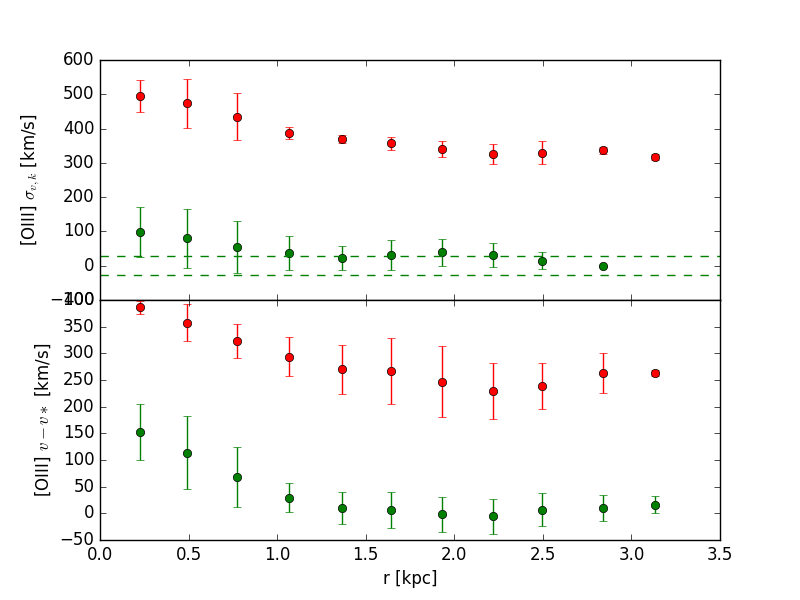
\includegraphics[width=.5\linewidth]{Plots/JO135_vvd2.png}& 
		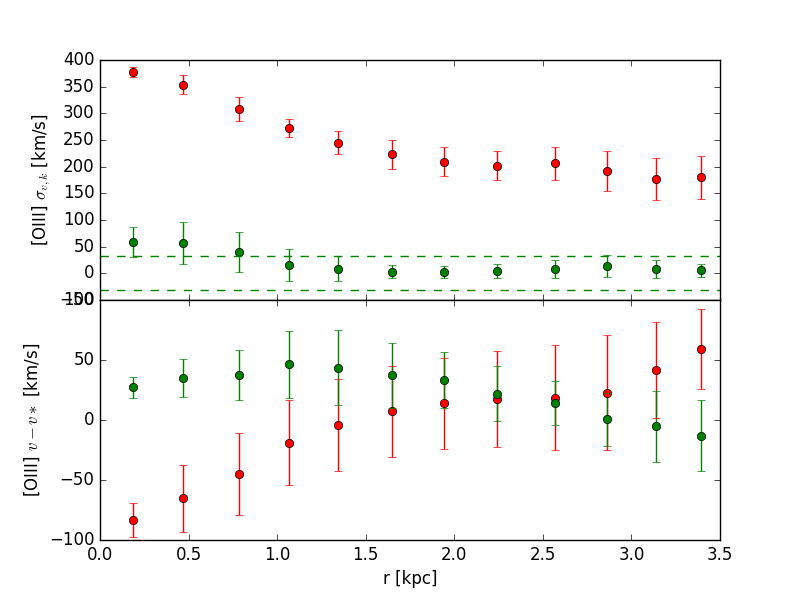
\includegraphics[width=.5\linewidth]{Plots/JO201_vvd2.png}\\
		JO204 & JW100\\
		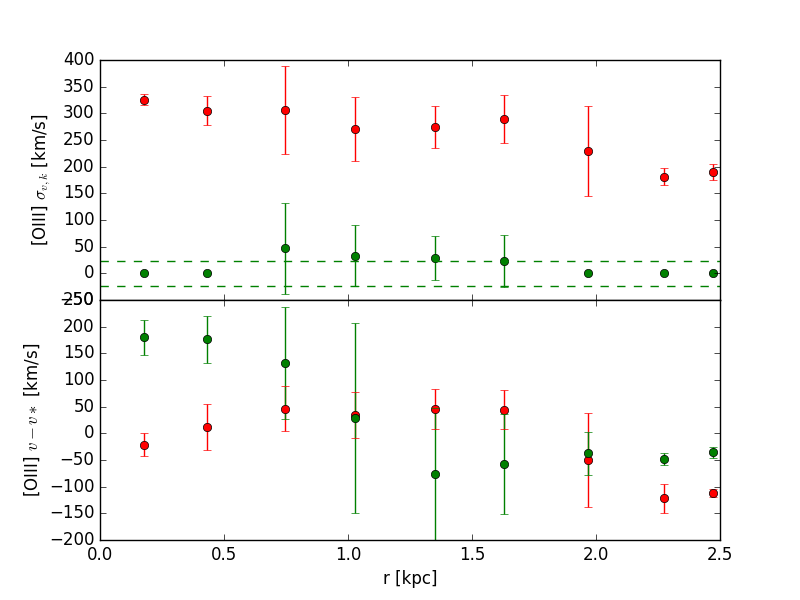
\includegraphics[width=.5\linewidth]{Plots/JO204_vvd2.png} &
		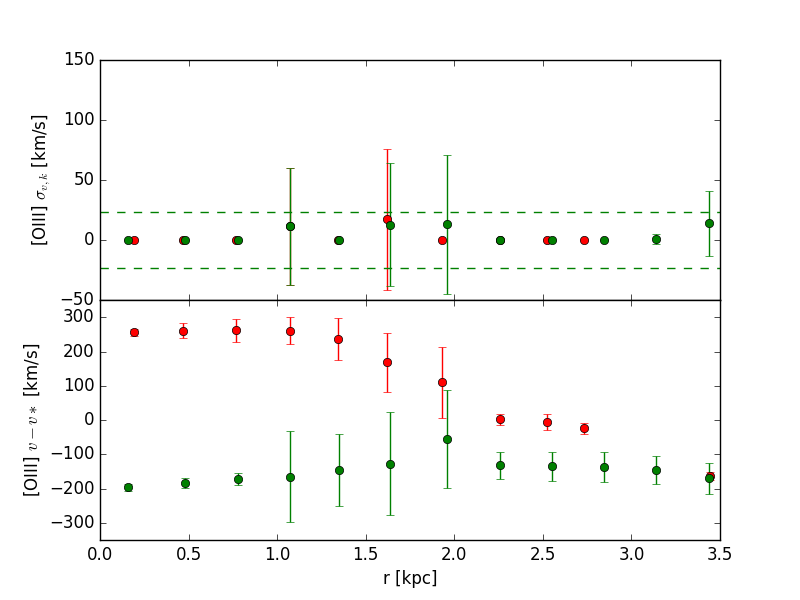
\includegraphics[width=.5\linewidth]{Plots/JW100_vvd2.png}\\
		%		JO206\\ 
		%		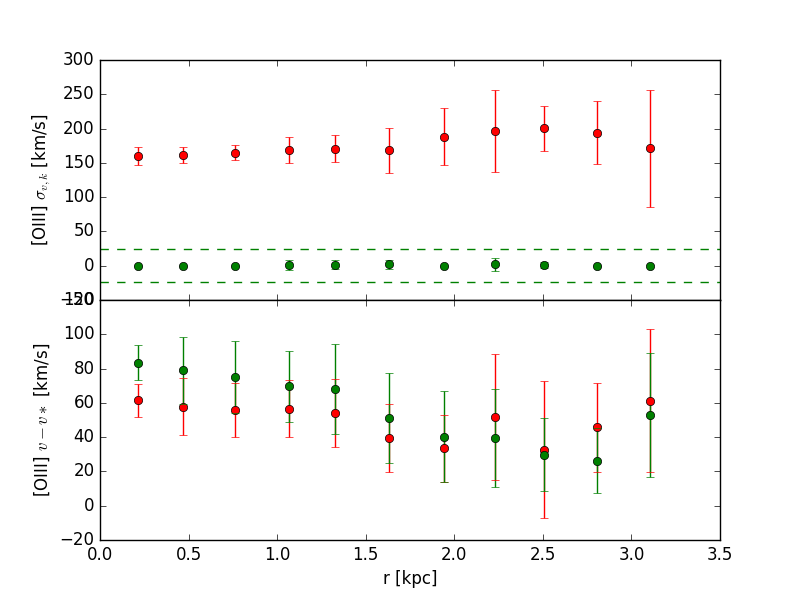
\includegraphics[width=.5\linewidth]{Plots/JO206_vvd2.png}\\
	\end{tabular} 
	\caption{Velocity and velocity dispersions of the narrow (green) and broad (blue)
		components of [OIII]$\lambda$5007. For the velocity dispersion, a value of 0 was assigned if the velocity dispersions was lower than the stellar velocity dispersions, that was subtracted in quadrature.\label{fig:vvd}}
\end{figure*}






%\noindent {\bf JO201}, or Kaz 364 [\citet{2017ApJ...844...49B},\citet{2018MNRAS.479.4126G}]
%was classified  by \citet{2009ApJ...707.1691A} as an AGN based on XMM observations.
%The analysis of the kinematic properties in the extranuclear regions of JO201 %\citep{2017ApJ...844...49B} revealed the presence of a redshifted, broad component in %H$\alpha$  up to $r \sim 50$ kpc fom the nucleus, a clear signature of ram-pressure %stripping that produces the large tails extending from the disk. Strong star formation was %also detected  both in the disk and along the tails \citep{2018MNRAS.479.4126G}. 

\citet{2013MNRAS.436.2576L,2015ApJS..221....9L}
%\citep{2016ApJ...824...50D}
%Strong FeVII 6087
%At high ionization parameters (log U … −1.5), Compton
%heating in the leading edge of the photoionized plasma
%becomes important, and the electron temperature rises to
%105 K or even higher. The clearest indicator of the presence of
%such highly ionized gas is coronal emission lines. Coronal lines
%are often weak but are found in the nuclear spectra of many of
%the S7 targets (Dopita et al. 2015), indicative of very high
%ionization parameters close to the central AGN. We do not
%accurately model the coronal line region and therefore we are
%unable to compare the observed and predicted coronal line
%strengths. The diffuse ionizing spectrum produced in the
%Compton heated zone is re-absorbed by the cooler plasma at
%larger radii.

%\noindent {\bf JO204} [\citet{2017ApJ...846...27G}] was included by \citet{2016ApJ...832...67N} in a sample of 71 double-peaked AGN selected from the SDSS and classified as an AGN with an outflow. 




 
 

%No blueshifted broad component is visible, which in the case of biconical outflows would imply that the approaching side of the outflow is absorbed by dust \citep{2010ApJ...708..419C}. 

%\noindent {\bf JW100}, or IC 5337, was classified as an AGN by \citet{2008ApJ...682..155W}, based on X--ray Chandra observations.   
%VO ratios and velocity parameters for each of them are displayed in  Fig.\ref{fig:vo_nb} and  Fig.\ref{fig:vvd}. 

%These properties, and the fact that the redshifted component is brighter in [OIII] than the blueshifted one, suggest that they are produced in an outflow: in the redshifted component we see the inner, ionized part of the clouds, with VO line ratios typical of an AGN, while in  the blueshifted part we mostly see the non-ionized regions \citep[see e.g.][]{2015ApJ...806...84L}.

 \citep[see e.g.][]{2015ApJ...806...84L}


\subsection{Outflows: mass and energy}

We computed the mass related to the outflow as \citep{2015A&A...580A.102C}
$M_{\rm out} = 8 \times 10^7 M_\odot C \frac{L[OIII]}{10^{44} erg s^{-1}}/\frac{<n_e>}{500 cm^{-3}}^{-1}$, with $C=\left<n_e\right>^2/\left<n_e^2\right> \sim ~ 1$. A typical density $\left<n_e\right> = 500$ cm $^{-3}$ was assumed.
The outflow kinetic energy is $E_{\rm kin} = \frac{1}{2} M_{\rm out} v^2_{\rm out}$, $v_{\rm out}$ being the bulk velocity of the outflow. As discussed e.g. in \cite{2016ApJ...833..171K}, different choices to estimate $v_{\rm out}$ were made in literature, reflecting different strategies to take into account geometrical effects (e.g. projection, opening angle of the outflow). Here we adopt the approximation \citep{2016ApJ...833..171K, 2018NatAs...2..198H} $v_{\rm out} = v^2_{\rm rad} +  \sigma^2$, where $v_{\rm rad}$ is the measured radial velocity and $\sigma$ the velocity dispersion measured from the broad component of [OIII]$\lambda$5007: following  \cite{2016ApJ...833..171K}, the velocity dispersion was corrected for the contribute from the gravitational potential by subtracting in quadrature the stellar velocity dispersion.  The size of the outflow, $r_{\rm out}$, was estimated from Fig.~\ref{vvd} as the radius where the velocity and velocity dispersions of the broad component merge with the stellar values. Again following \cite{2016ApJ...833..171K}, from the mean bulk velocity and the size of the outflow we can then derive the outflow lifetime, $t_{\rm out} = r_{\rm out}/\bar{v}_{\rm out}$, and the  outflow mass rate, $\dot{M}_{\rm out}=M_{\rm out}/t_{\rm out}$ and energetic rate,$\dot{E}_{\rm kin}=E_{\rm kin}/t_{\rm out}$ .
\citet{2015A&A...580A.102C} derived for a sample of AGN the outflow efficiency, defined as $\eta =  \dot{E}_{\rm kin}/L_{\rm AGN}$, where $L_{\rm AGN} = 3500 L_{\rm[OIII]}$ erg/s \citep{2004ApJ...613..109H} estimates the bolometric luminosity of the AGN. We emphasize all the uncertainties  related both to the outflow kinetic energy and the rough estimate of the bolometric luminosity. Nevertheless, consistently with the results in\citet{2015A&A...580A.102C},  for all galaxies we obtain $\eta \ll 0.01\%$, suggesting that the outflow is not impacting the host galaxy environment.

%In order to see whether different ionization mechanisms may produce the broad and narrow line components \citep[see e.g.][]{2018A&A...617A.139S}, we analyzed (Fig.\ref{fig:vo_nb}) the VO diagrams for those spaxels where a reliable decomposition can be achieved for all the VO lines. We emphasize that the physical meaning of the decomposition should be taken with care since in some cases the best-fitting solution may not be unique, in particular as the components are strongly blended The result is  displayed in Fig.\ref{fig:vo_nb} for spaxels within 2 kpc from the nucleus: it appears that, similarly to what observed for the redshifted component in JW100, for JO135, JO201 and JO206  the broad component lies in the high-excitation part of the VO diagram, while for the narrow component extends to the HII region, probably due to an increasing contribute from SF regions. 
%In JO204, [OIII]$\lambda$5007/H$\beta$ is higher in the narrow component than in the broad one. Finally, the width of the narrow component is close to the stellar velocity dispersion, and not compatible with the presence of fast shocks: since narrow line ratios occupy the same region in the VO diagram as the broad line ratios, this further rules out shocks as a dominant ionization mechanism in the nuclear regions.



\section{Conclusions}

In this paper we confirmed the presence of an AGN  in at least five of the seven jellyfish galaxies presented in \citep{2017Natur.548..304P}. While shocks can certainly play a role in the ionization of the gas, we showed that they can't explain the line ratios observed in the nuclear regions, more typical of AGN. The same galaxies also present complex emission line profiles, with at least two components with different widths. The narrow component shows kinematical properties in agreement with virialized gas, while the broad component indicates the presence of outflowing gas. 


We detect the presence of outflows in JO201,....: their extension is limited to few kpc around the nucleus, which suggests that they can hardly affect the large-scale properties of the galaxies \citep{2016ApJ...819..148K}. This would confirm that the AGN activity is triggered by the disturbed environment (e.g. via ram pressure), rather than ......

\section*{Acknowledgements}

%%%%%%%%%%%%%%%%%%%%%%%%%%%%%%%%%%%%%%%%%%%%%%%%%%

%%%%%%%%%%%%%%%%%%%% REFERENCES %%%%%%%%%%%%%%%%%%

% The best way to enter references is to use BibTeX:

\bibliographystyle{mnras}
\bibliography{paper} % if your bibtex file is called example.bib


%%%%%%%%%%%%%%%%%%%%%%%%%%%%%%%%%%%%%%%%%%%%%%%%%%

%%%%%%%%%%%%%%%%% APPENDICES %%%%%%%%%%%%%%%%%%%%%

\appendix



\section{Spectra and nuclear emission lines}
\label{app:spectra}

Fig.\ref{fig:spectra} shows the spectrum from the central spaxel in each galaxy; some emission lines are displayed in Fig.\ref{fig:emlines} for the galaxies with outflow signatures (JO201, JO204, JO135 and JW100).

\begin{figure*}
	\begin{tabular}{cc}
		JO135 &  JO201\\
		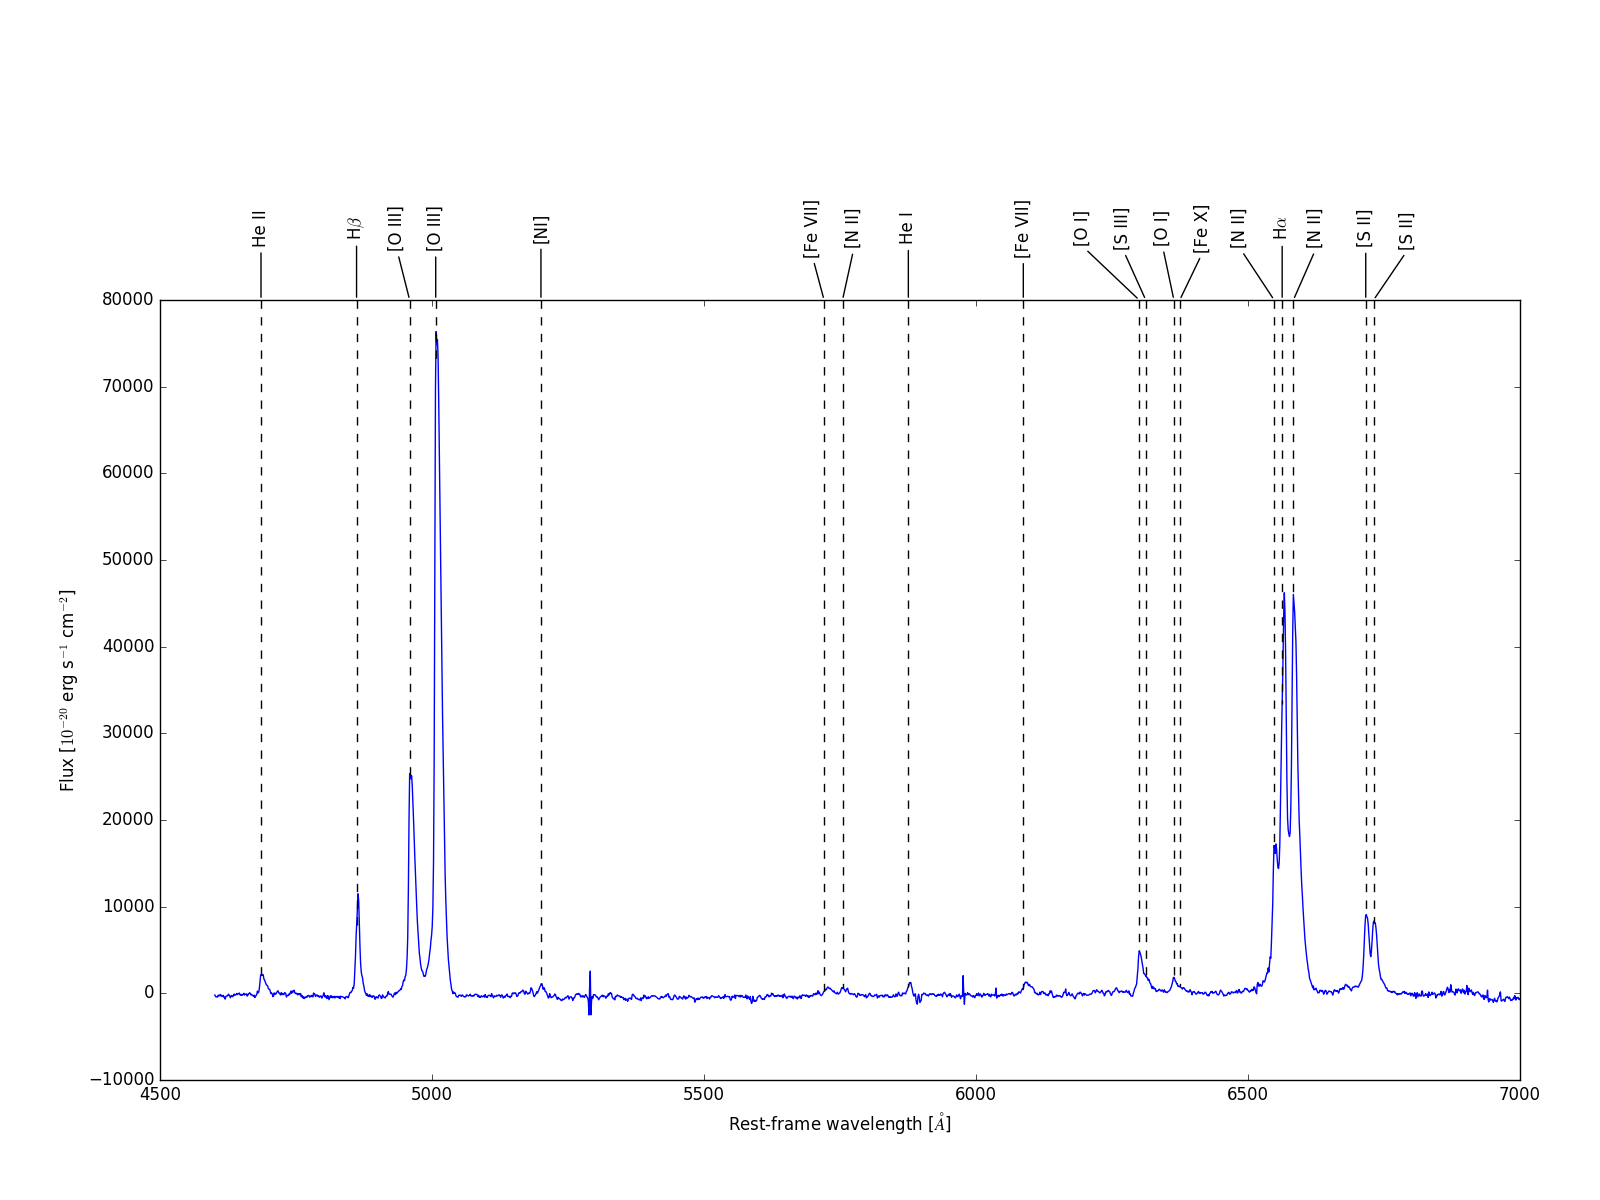
\includegraphics[width=.5\linewidth]{Plots/JO135_nucleus}	& 		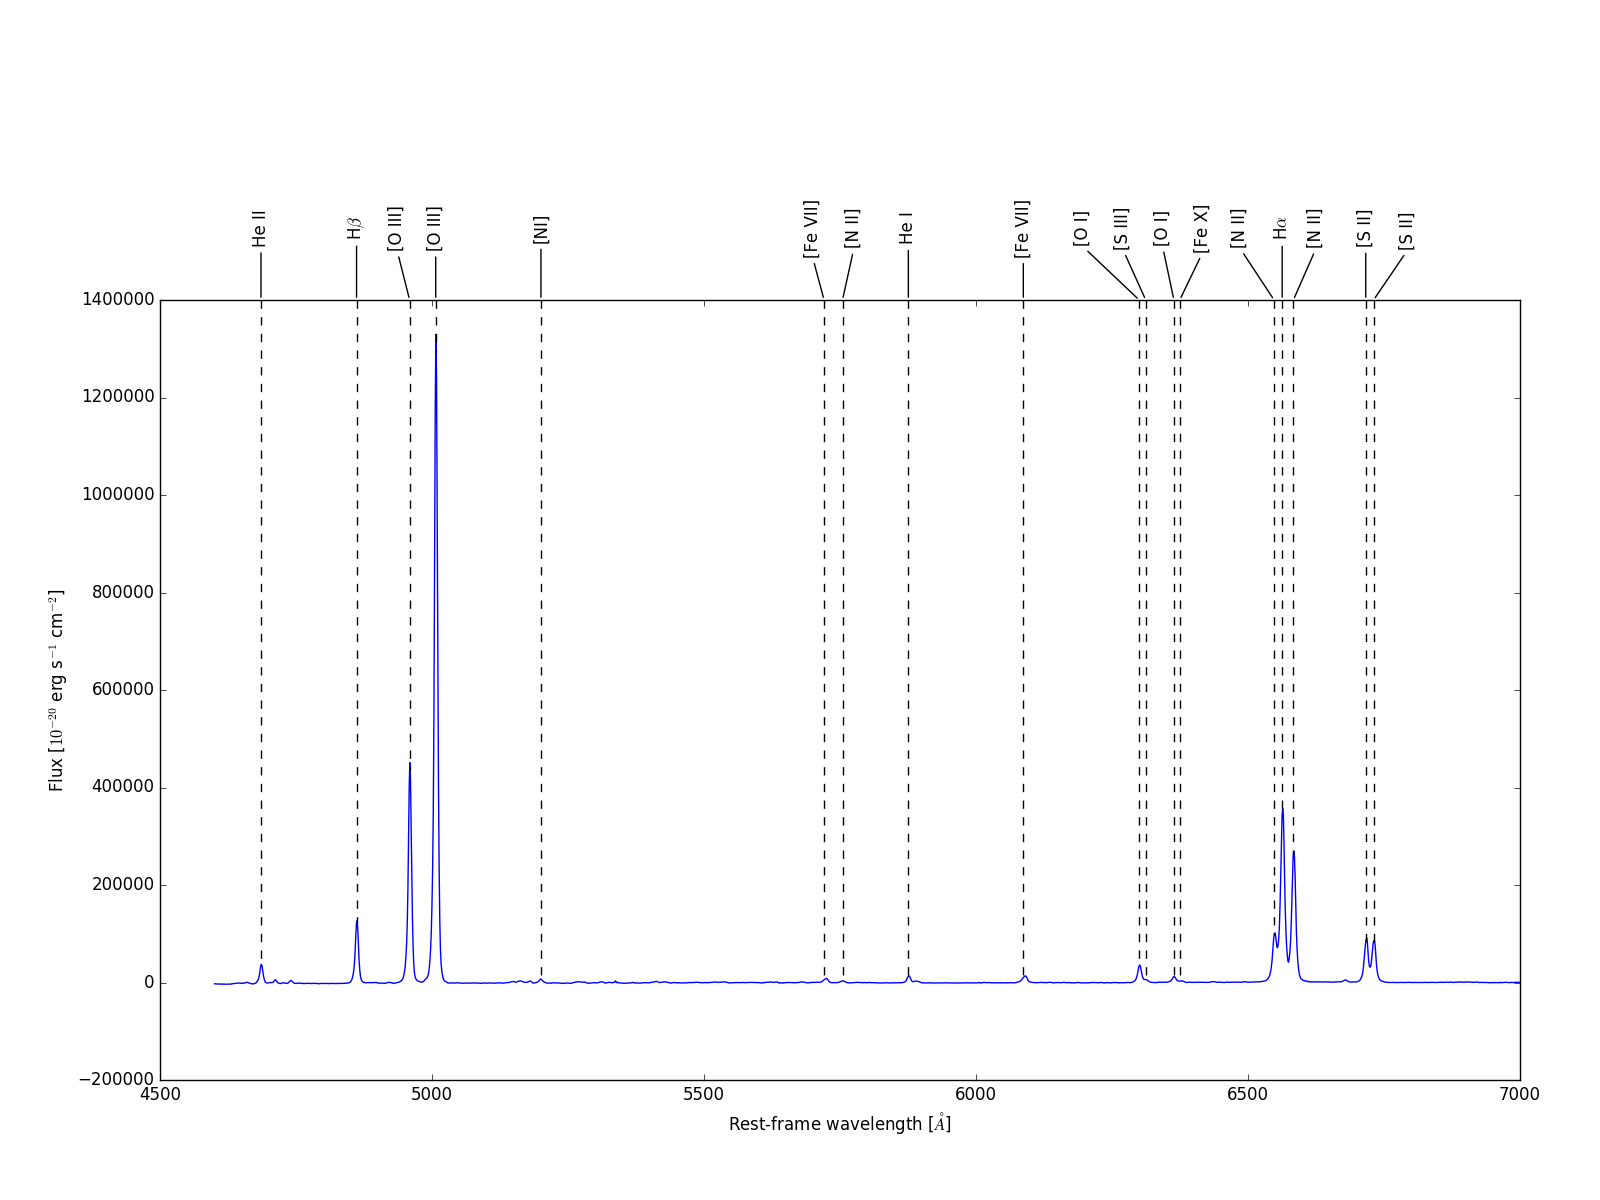
\includegraphics[width=.5\linewidth]{Plots/JO201_nucleus} \\
		JO204 &  JO206\\
		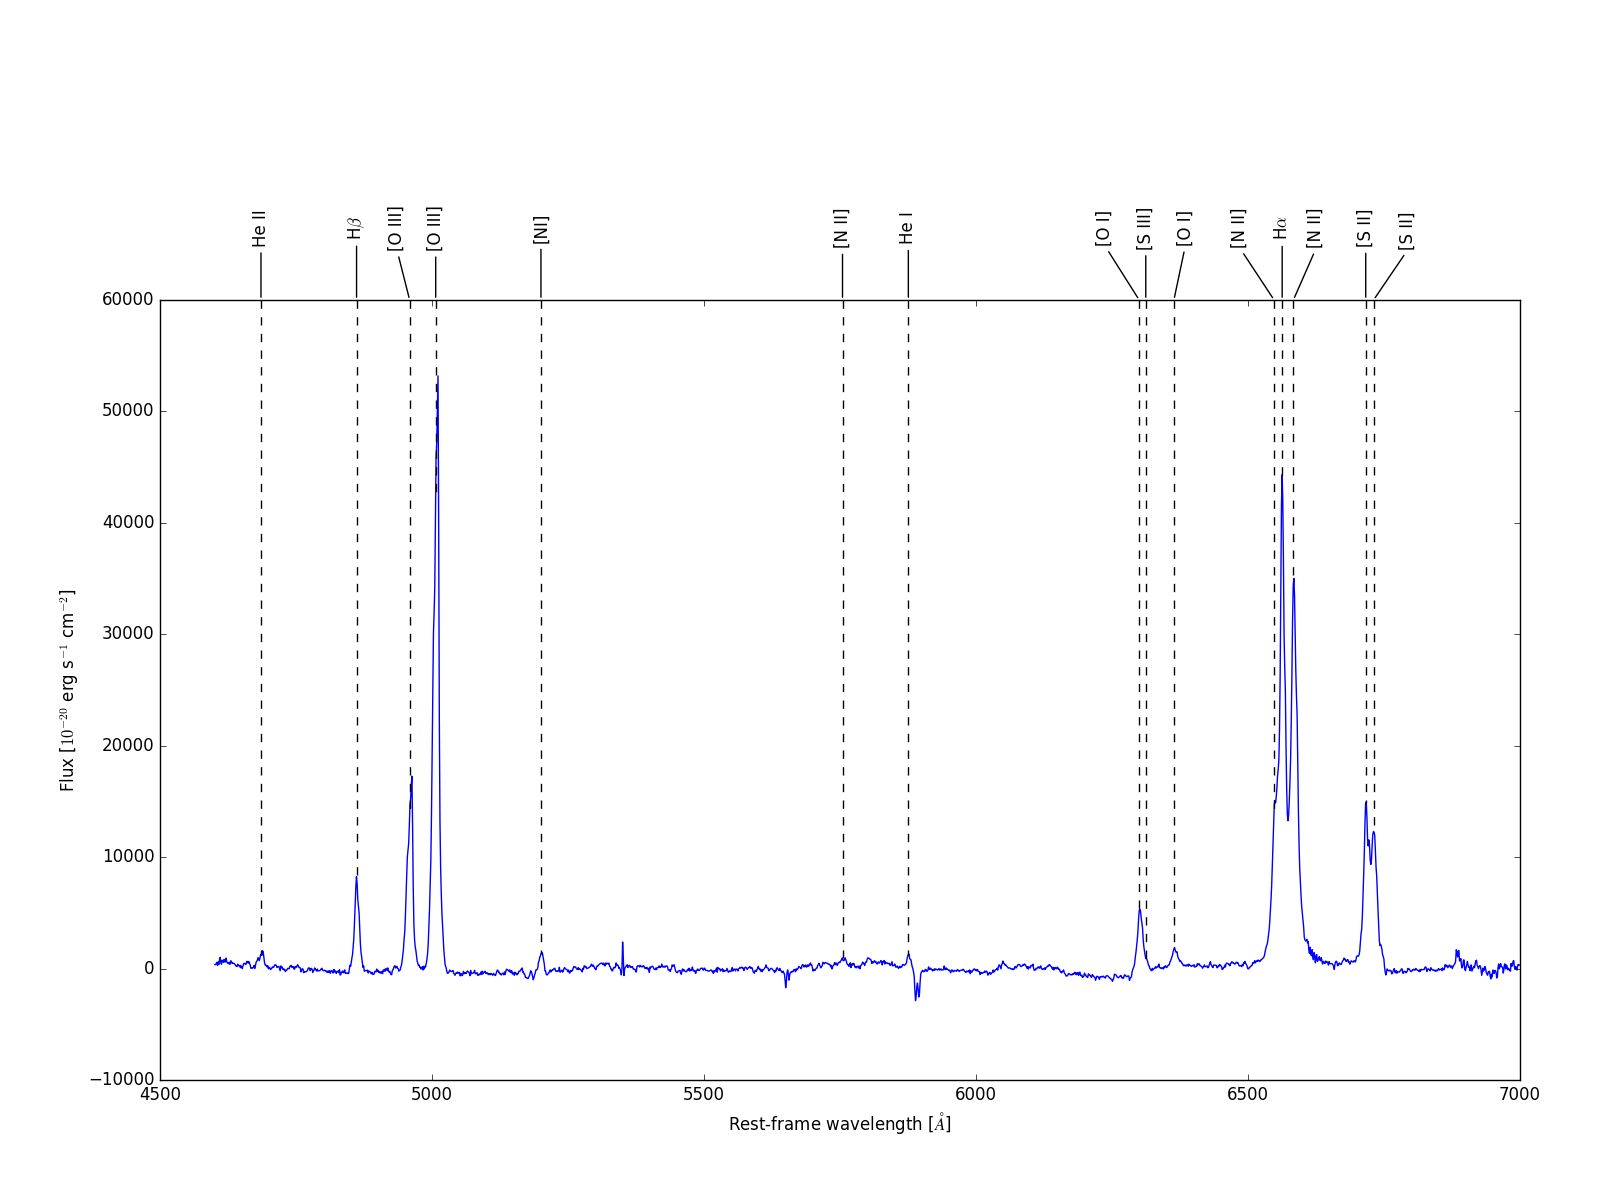
\includegraphics[width=.5\linewidth]{Plots/JO204_nucleus}&
		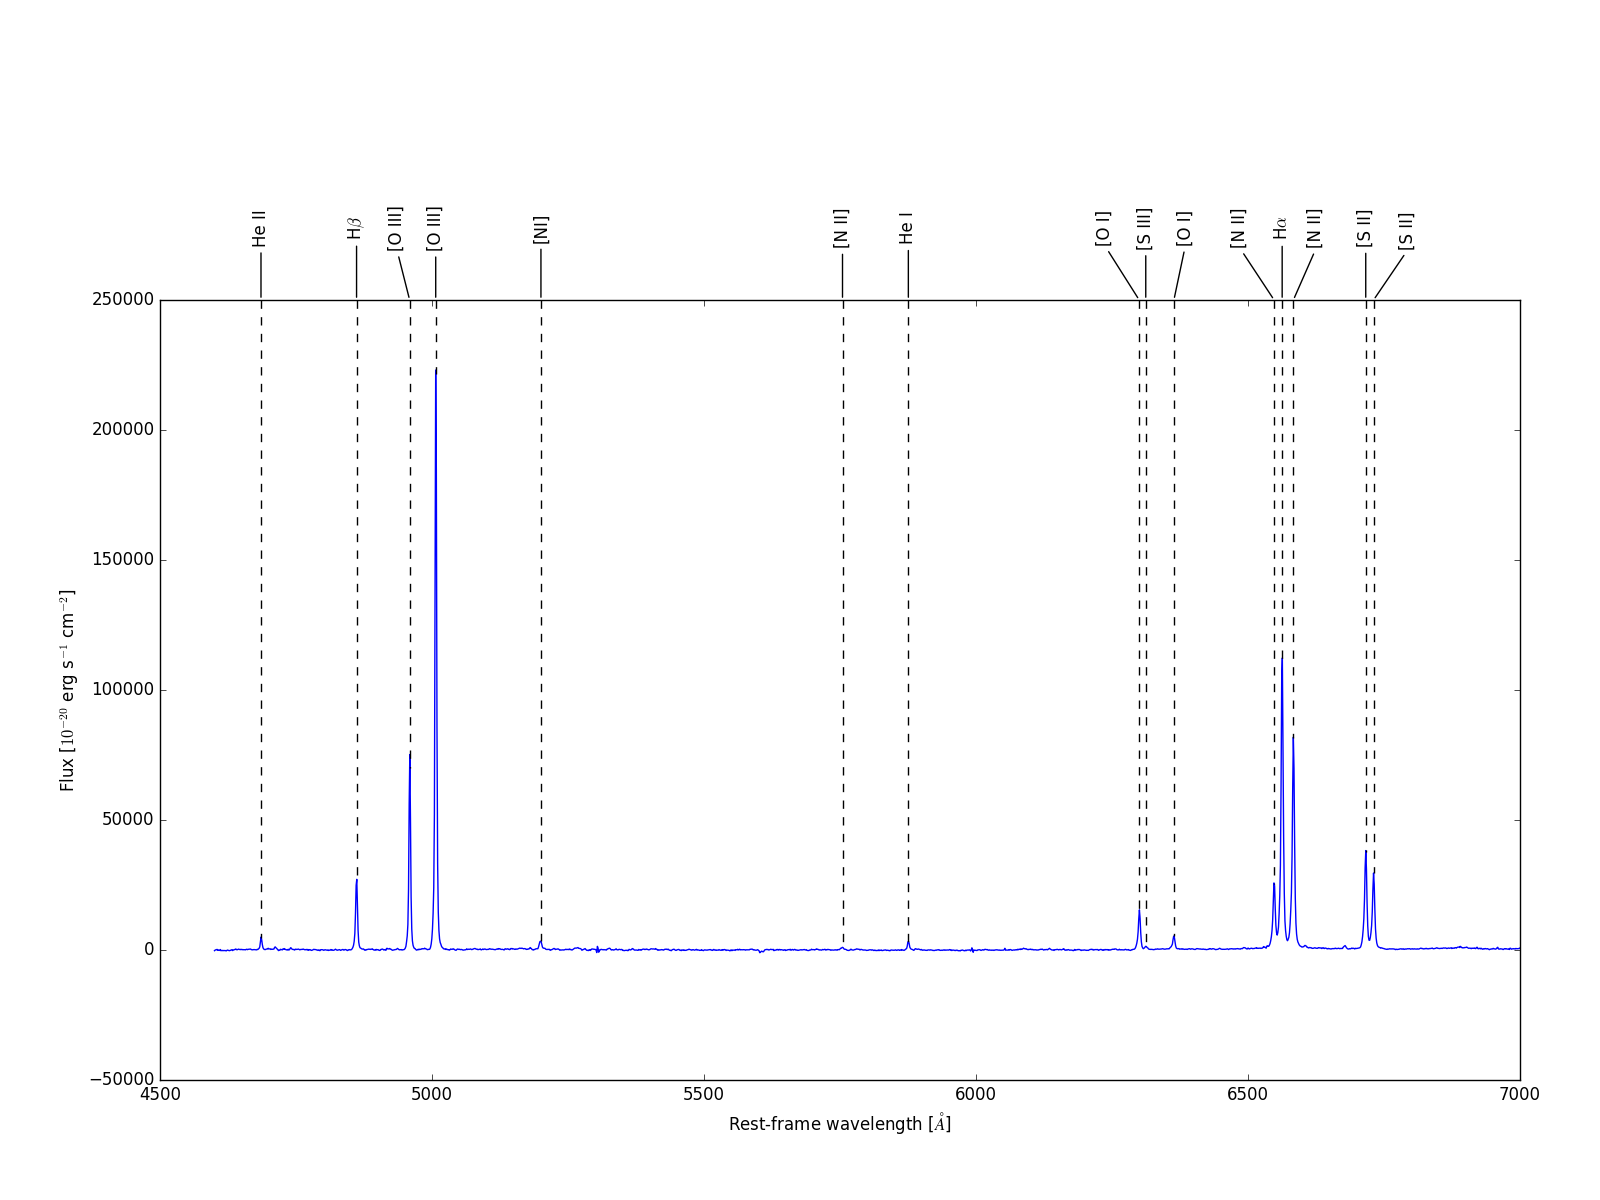
\includegraphics[width=.5\linewidth]{Plots/JO206_nucleus} \\
		JW100 &  JO175\\
		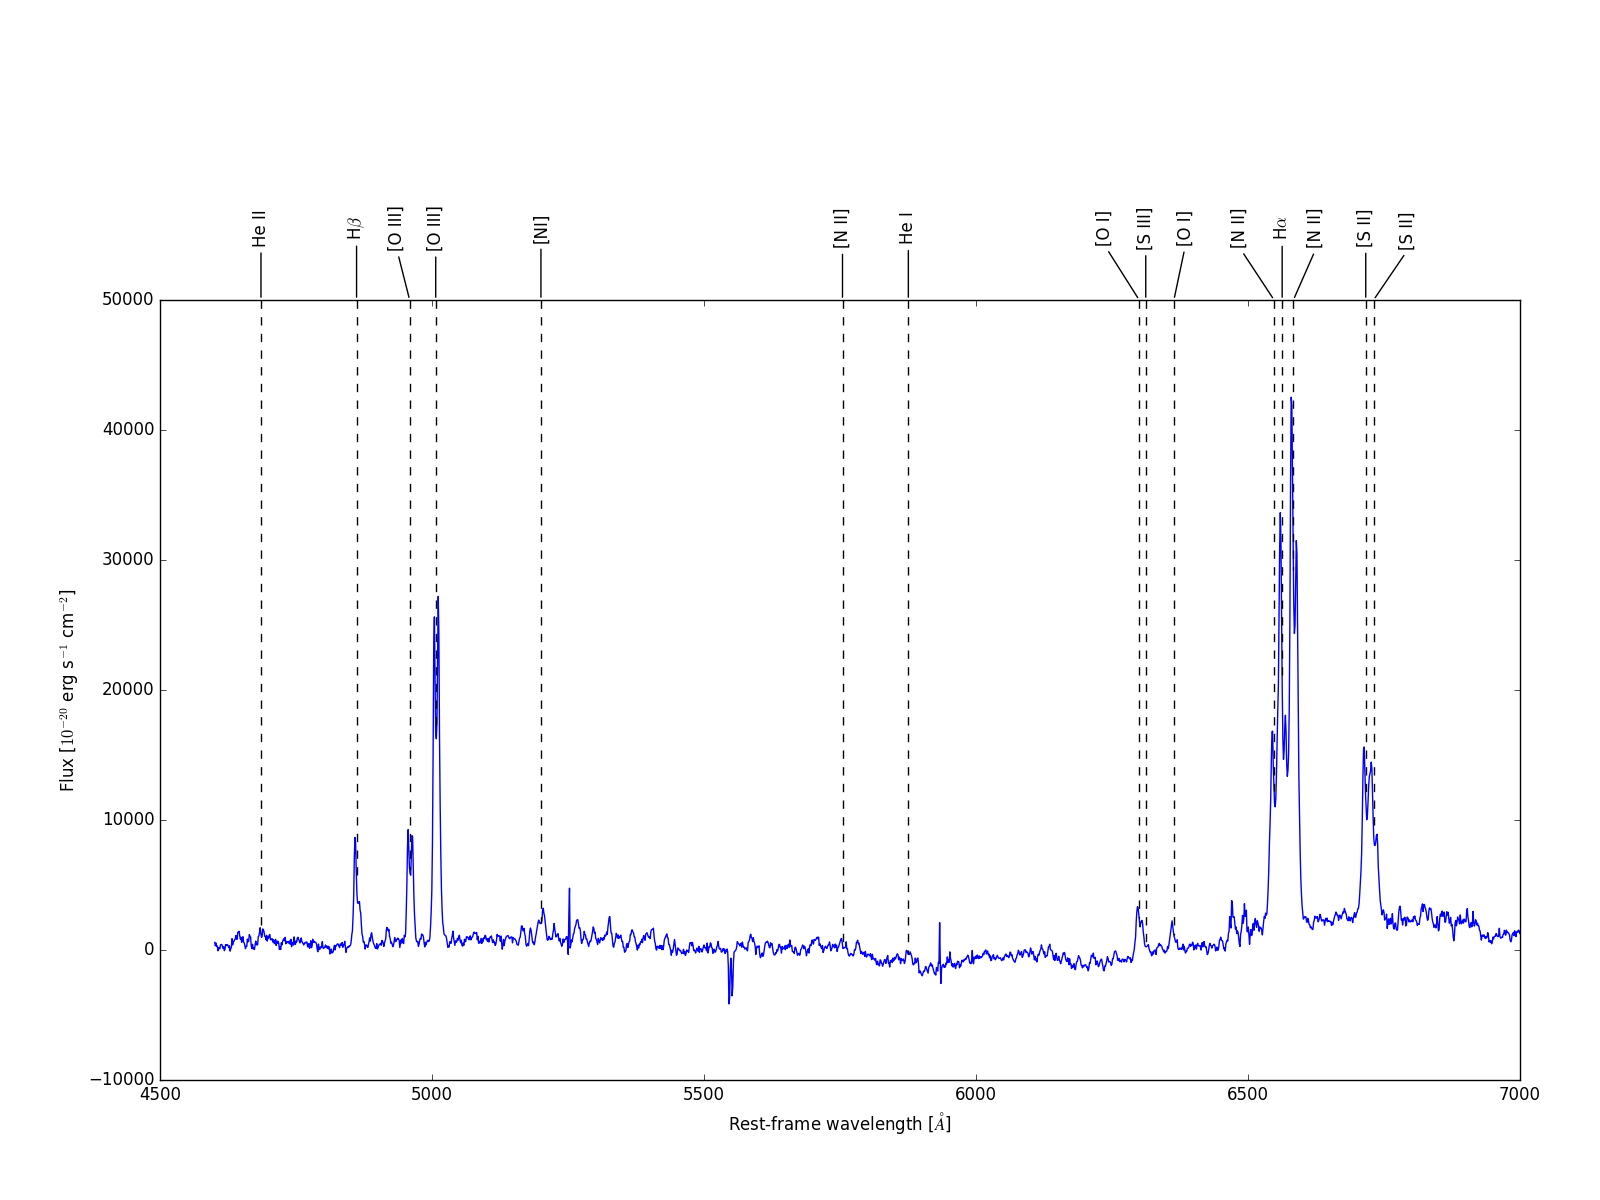
\includegraphics[width=.5\linewidth]{Plots/JW100_nucleus}&
		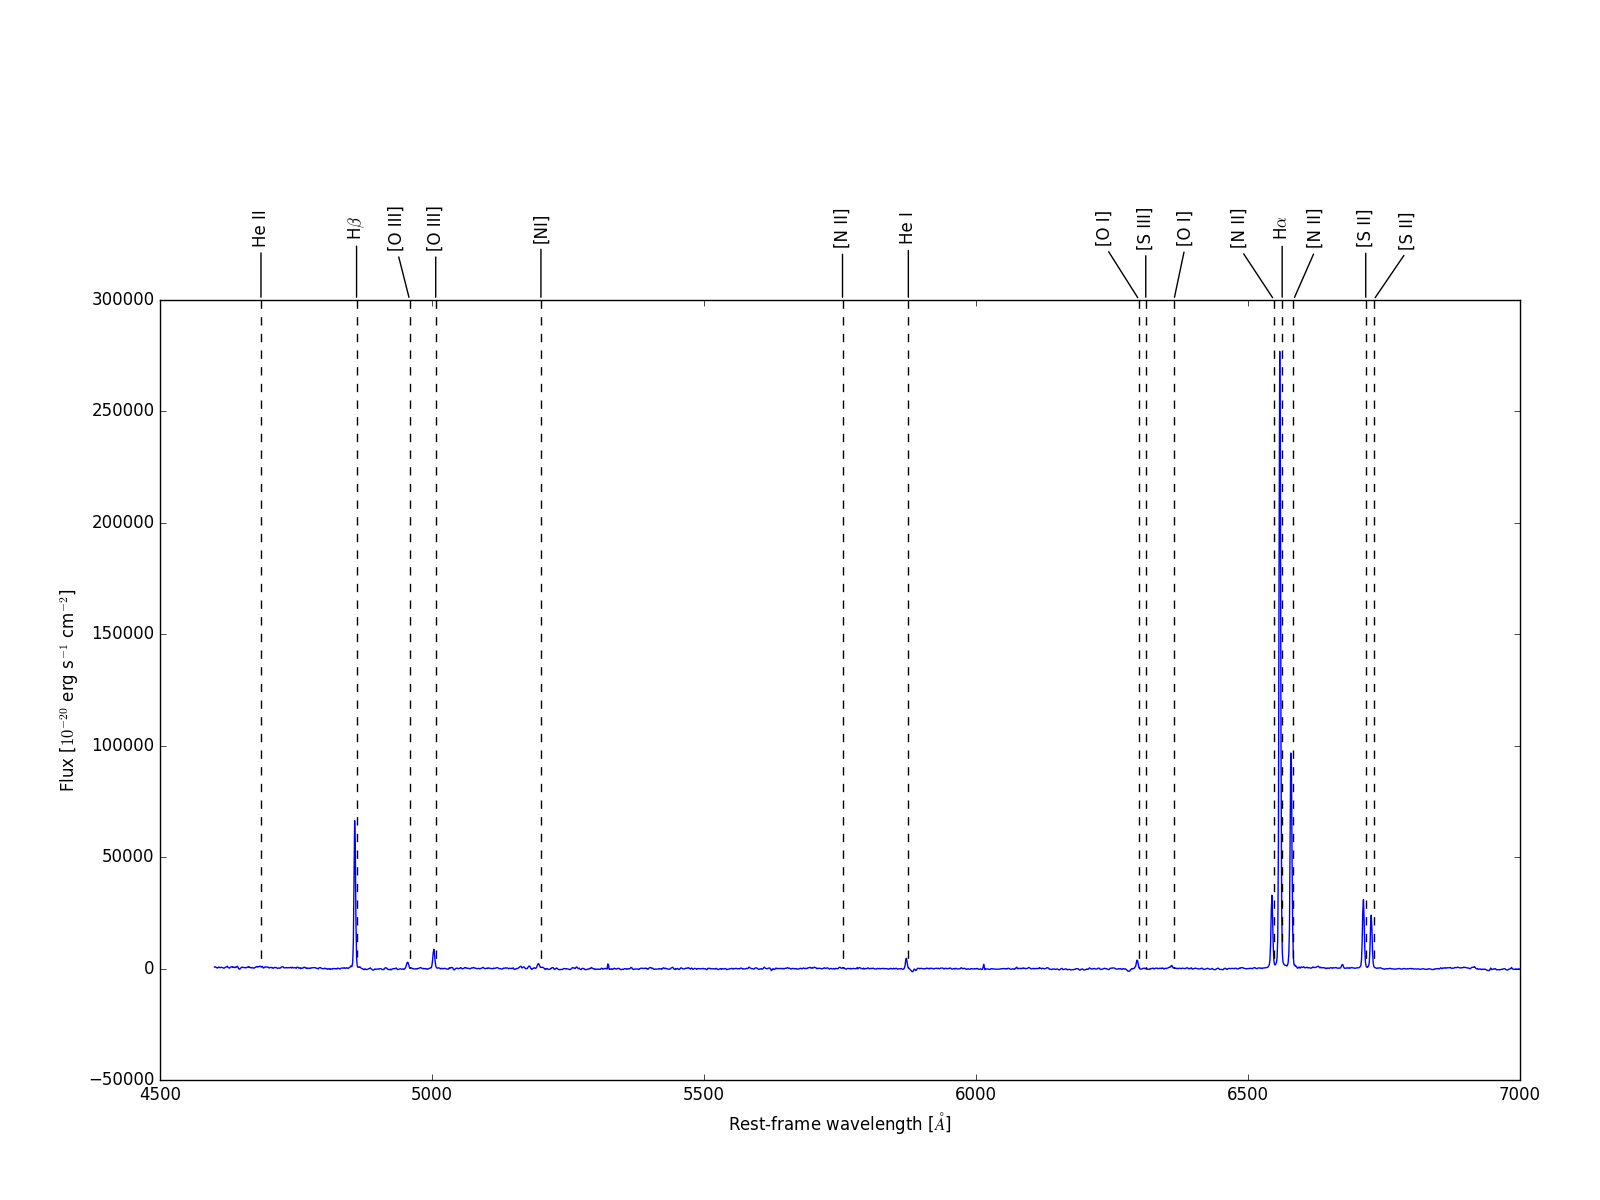
\includegraphics[width=.5\linewidth]{Plots/JO175_nucleus} \\
	\end{tabular} 
	\caption{Spectra in the central spaxels and line identifications.\label{fig:spectra}}
\end{figure*}


\begin{figure*}
	\begin{tabular}{cc}		
		JO194 & \\		
		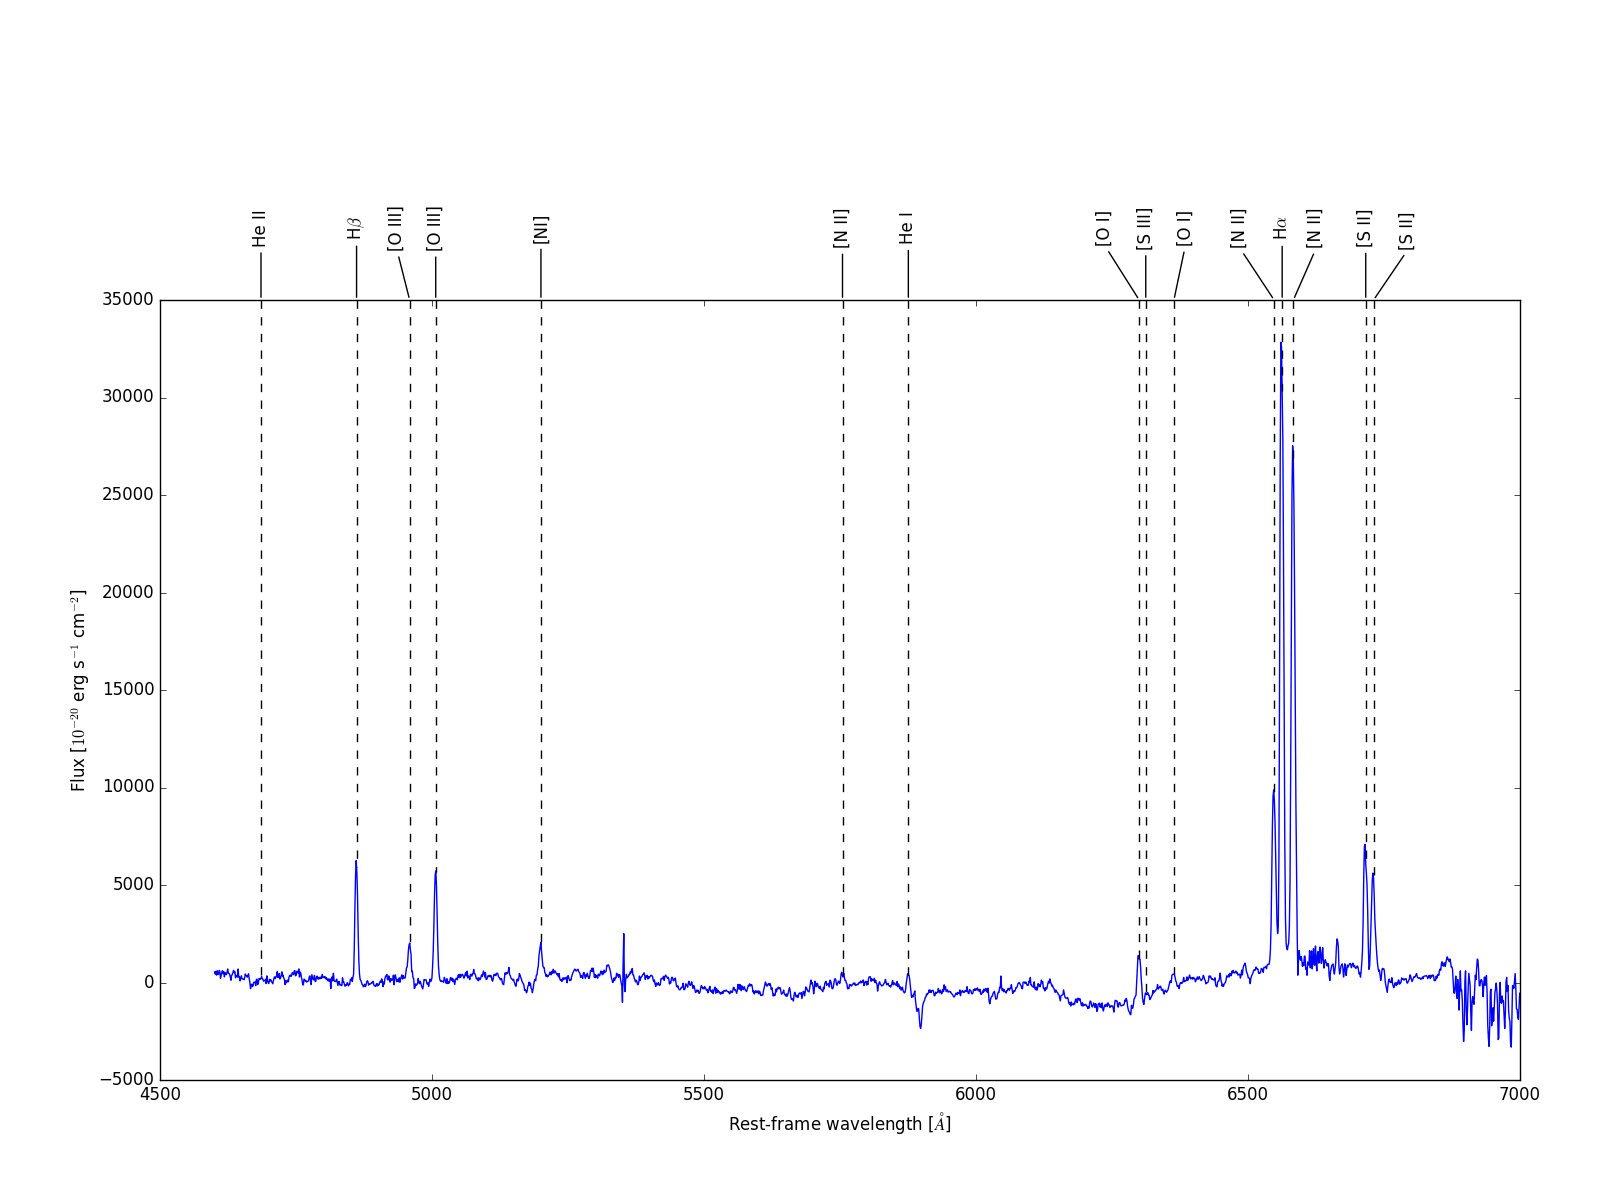
\includegraphics[width=.5\linewidth]{Plots/JO194_nucleus}& \\
	\end{tabular} 
	\contcaption{}
\end{figure*}


\begin{figure*}
	\begin{tabular}{cc}
		JO135 & JO201\\	
		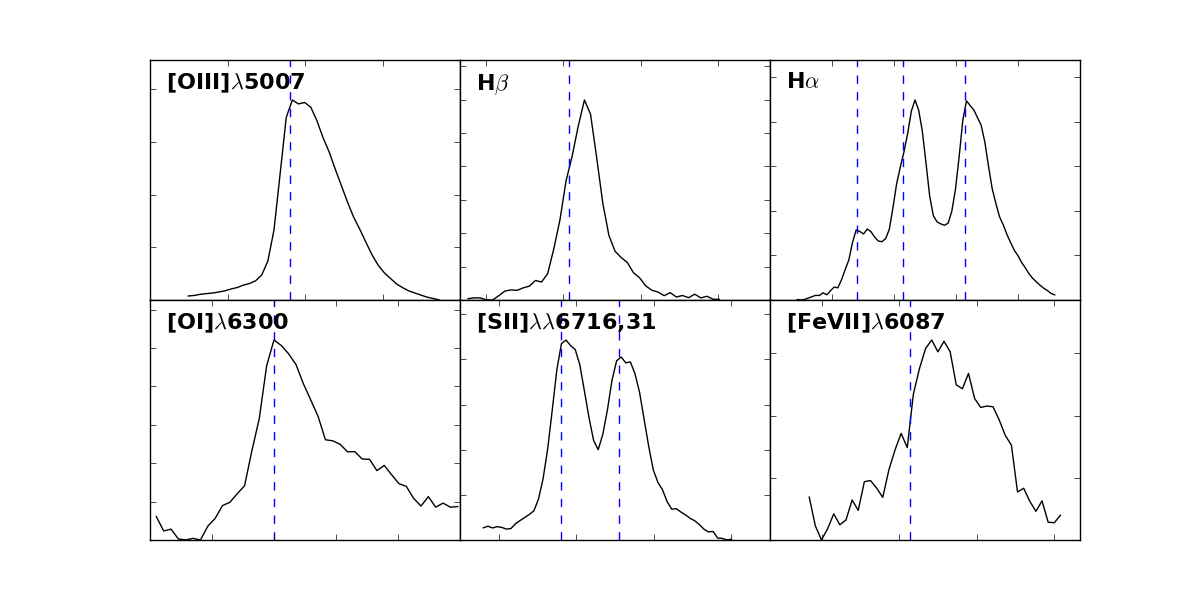
\includegraphics[width=.5\linewidth]{Plots/alines_peak_JO135}	& 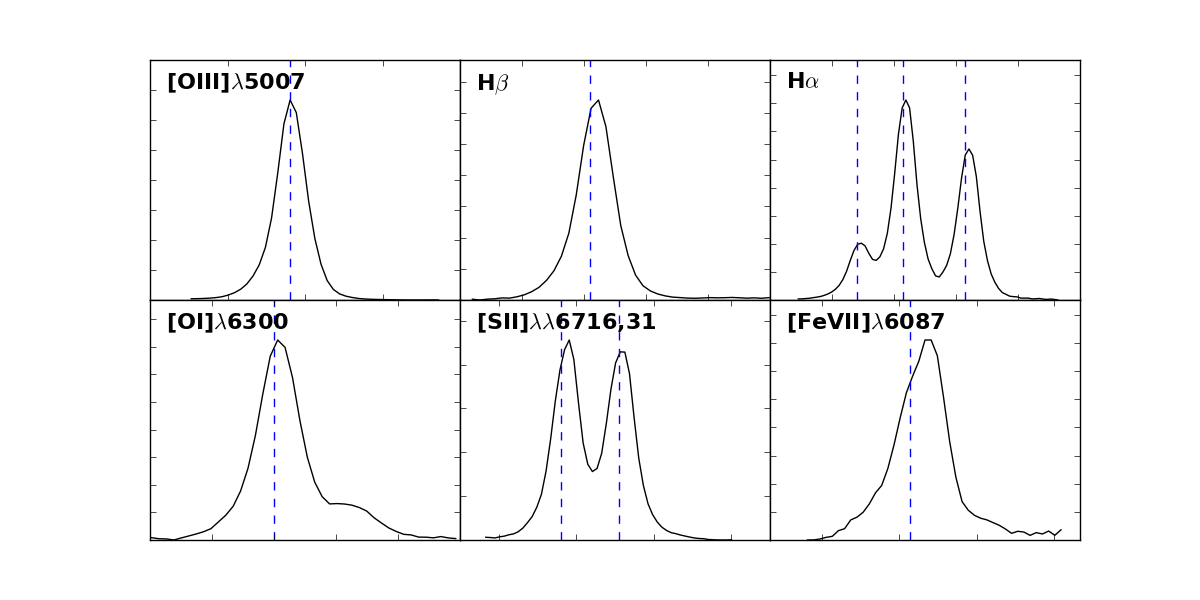
\includegraphics[width=.5\linewidth]{Plots/alines_peak_JO201} \\
		JO204 & JO206\\
		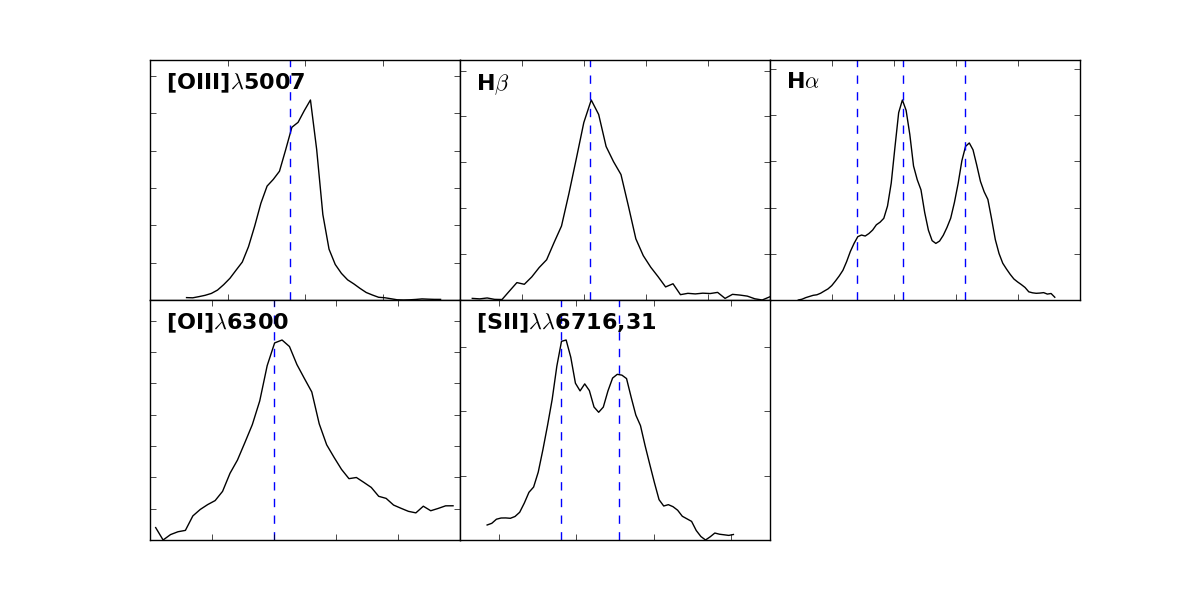
\includegraphics[width=.5\linewidth]{Plots/alines_peak_JO204}&
		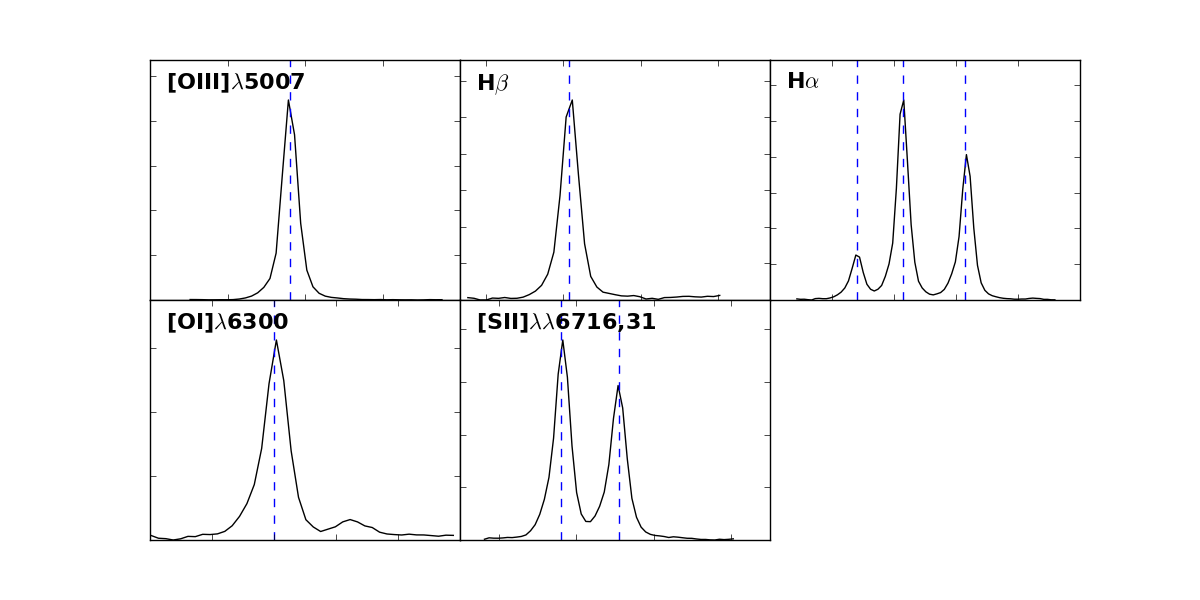
\includegraphics[width=.5\linewidth]{Plots/alines_peak_JO206}\\
		JW100 & JO175\\
		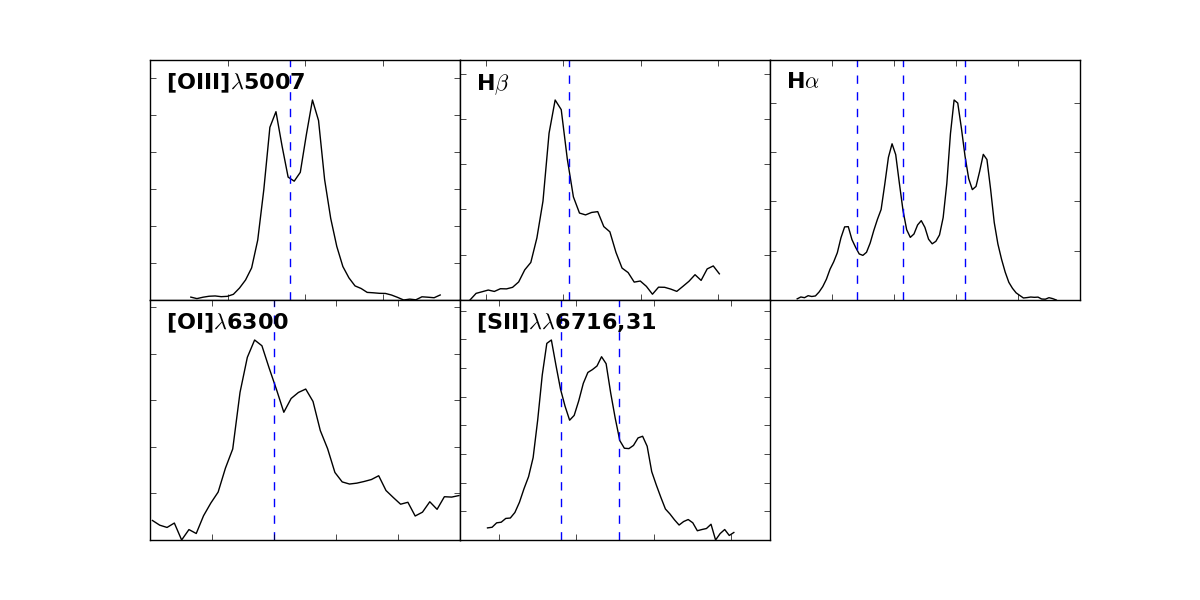
\includegraphics[width=.5\linewidth]{Plots/alines_peak_JW100} & 
		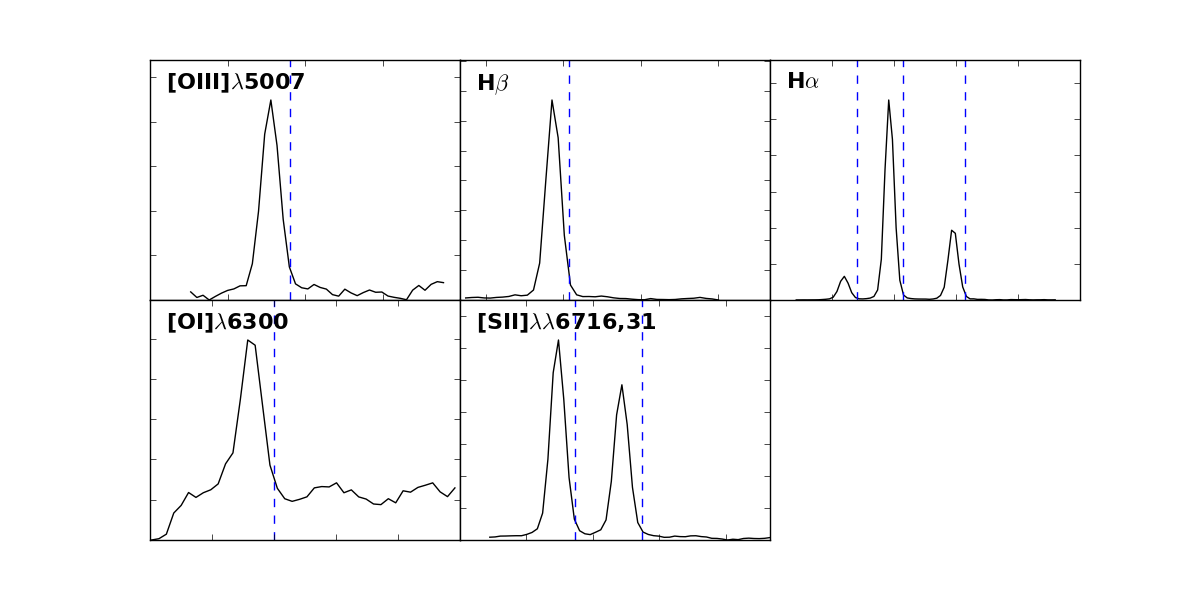
\includegraphics[width=.5\linewidth]{Plots/alines_peak_JO175}\\
		JO194&\\
		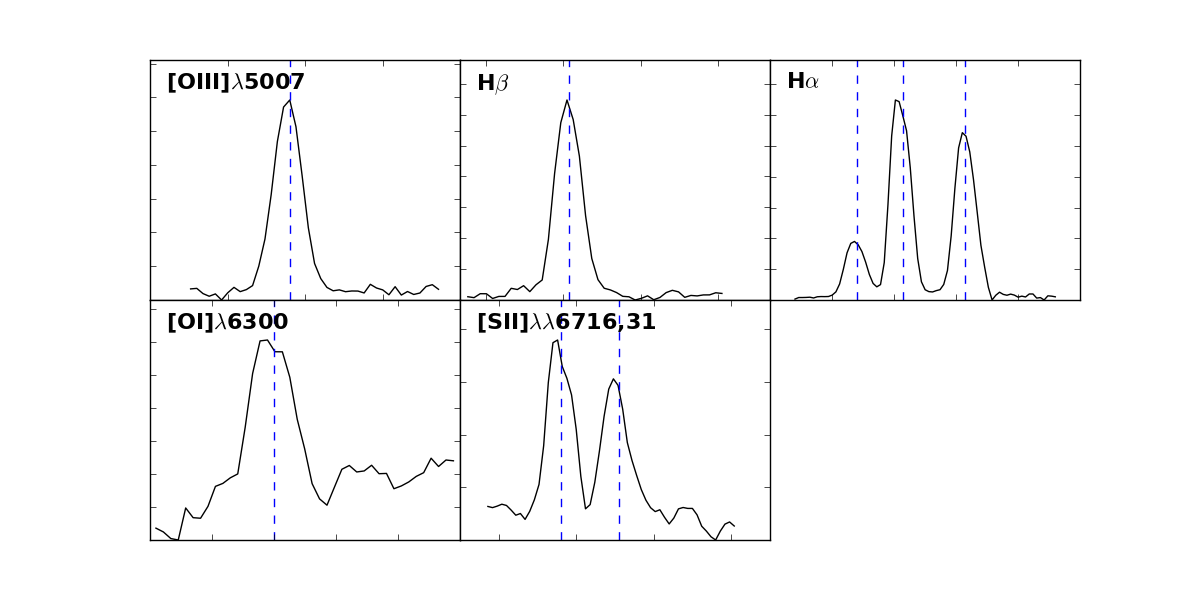
\includegraphics[width=.5\linewidth]{Plots/alines_peak_JO194} & \\				
	\end{tabular} 
	\caption{Emission line profiles in the central spaxel.\label{fig:emlines}}
\end{figure*}

\section{VO and model maps}
\label{app:class_maps}

Fig.\ref{fig:mapsKV2NB} compares the classification in HII-regions, Composite, AGN and Liners based on [NII]$\lambda$6583/H$\alpha$ vs. [OIII]$\lambda$5007/H$\beta$ as in \citet{2017Natur.548..304P}, with best-fit AGN and shock models derived with \texttt{NebulaBayes}.

\begin{figure*}
	\begin{tabular}{c}
		JO135 \\
		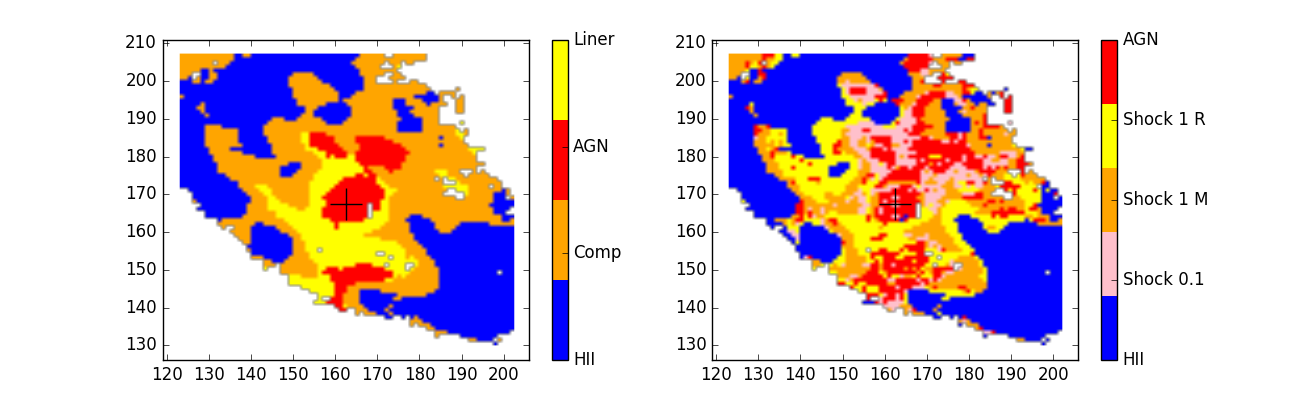
\includegraphics[width=.95\linewidth]{Plots/JO135_NB_xbest_grid.png}\\
		JO201\\
		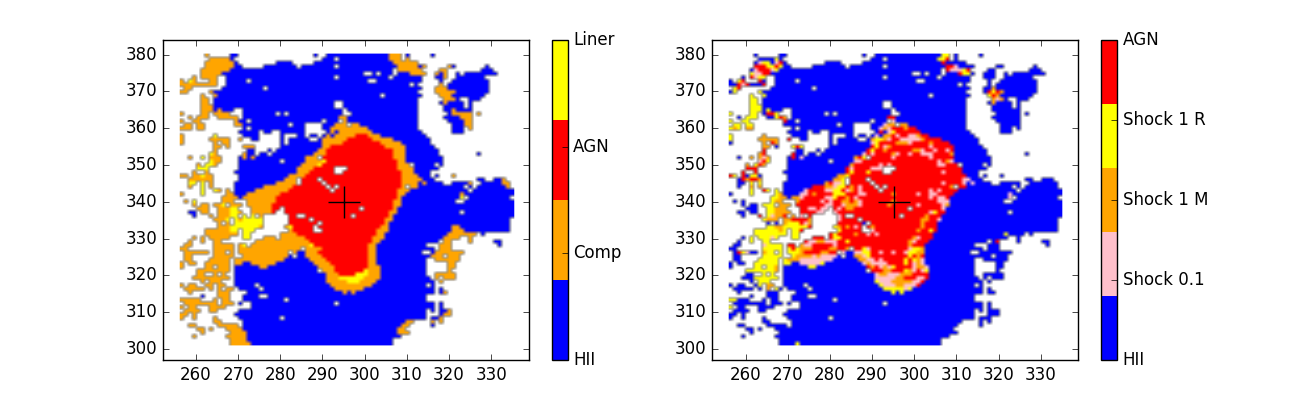
\includegraphics[width=.95\linewidth]{Plots/JO201_NB_xbest_grid.png}\\
		JO204\\
		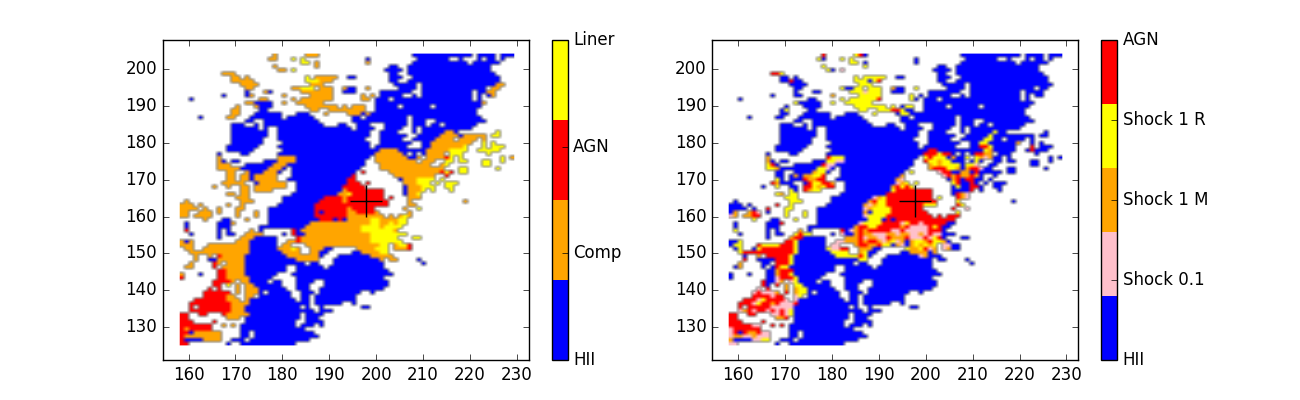
\includegraphics[width=.95\linewidth]{Plots/JO204_NB_xbest_grid.png}\\
		JO206 \\
		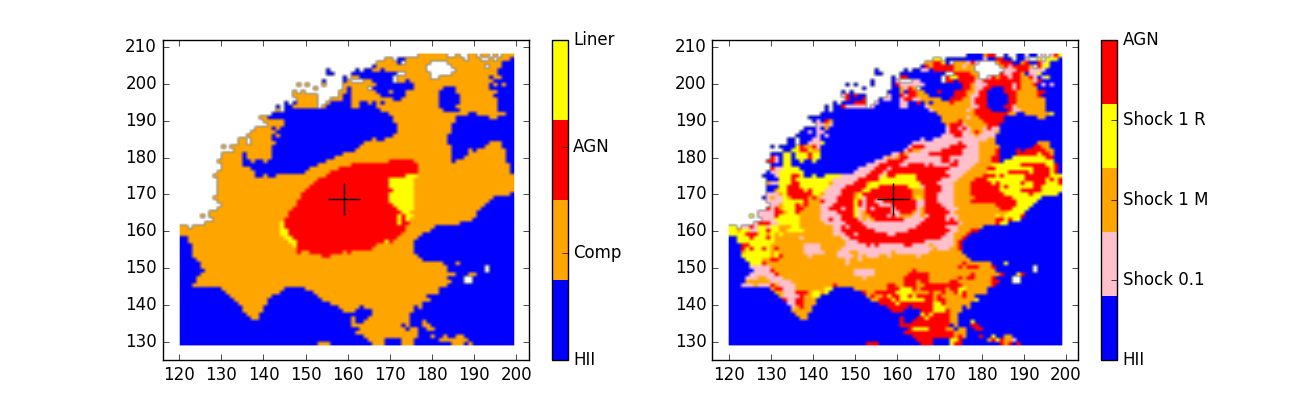
\includegraphics[width=.95\linewidth]{Plots/JO206_NB_xbest_grid.png}\\
	\end{tabular} 
	\caption{Color coded maps in the a region of 100x100 spaxels around the nucleus. {\em Left}: VO classification (1: HII, 2: composite, 3: AGN, 4: LINER). {\em Right:} NB models (1: HII; 2: $n=0.1$, solar; 3: $n=1$, solar; 4: $n=1$, 2x solar, 5: AGN). \label{fig:mapsKV2NB}}
\end{figure*}

\begin{figure*}
	\begin{tabular}{c}	
		JW100 \\ 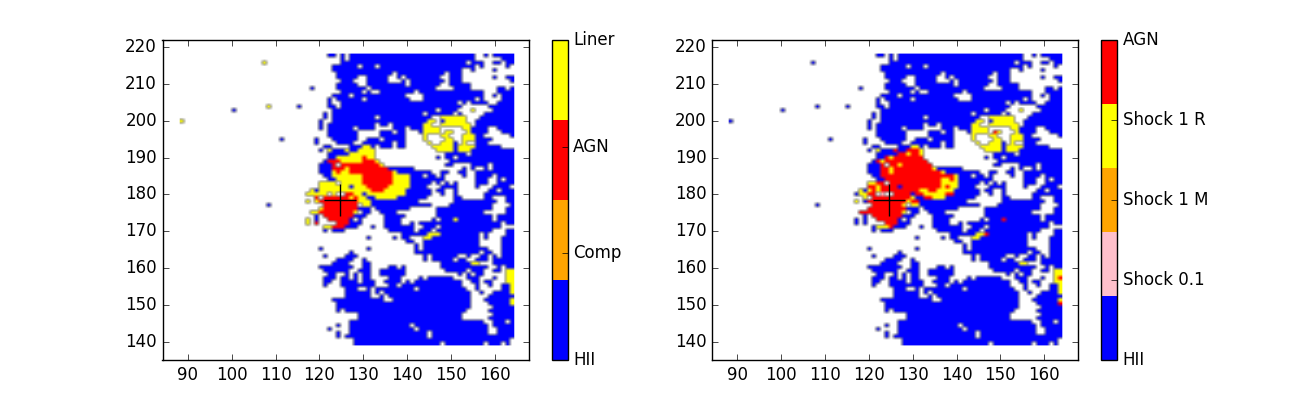
\includegraphics[width=.95\linewidth]{Plots/JW100_NB_xbest_grid.png}\\
		JO194 \\	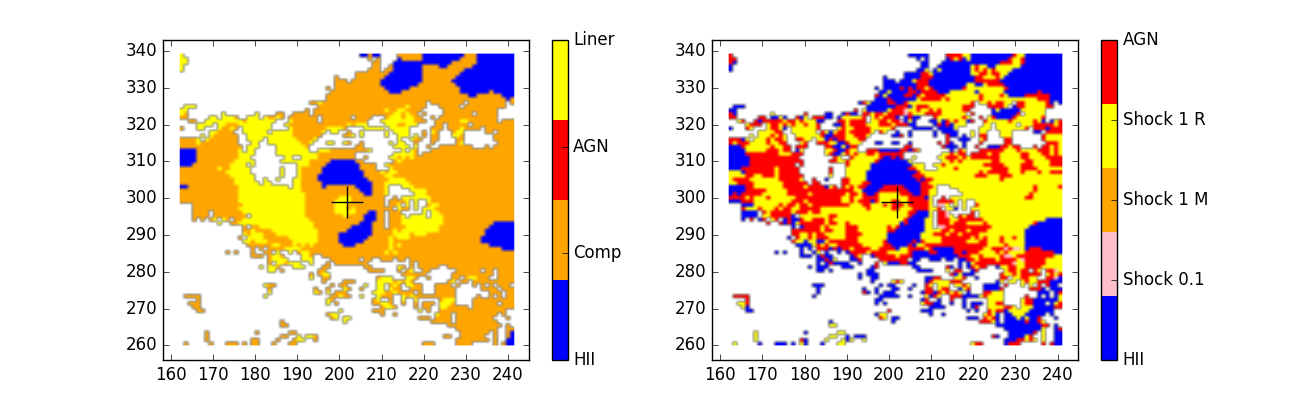
\includegraphics[width=.95\linewidth]{Plots/JO194_NB_xbest_grid.png}\\
		JO175 \\	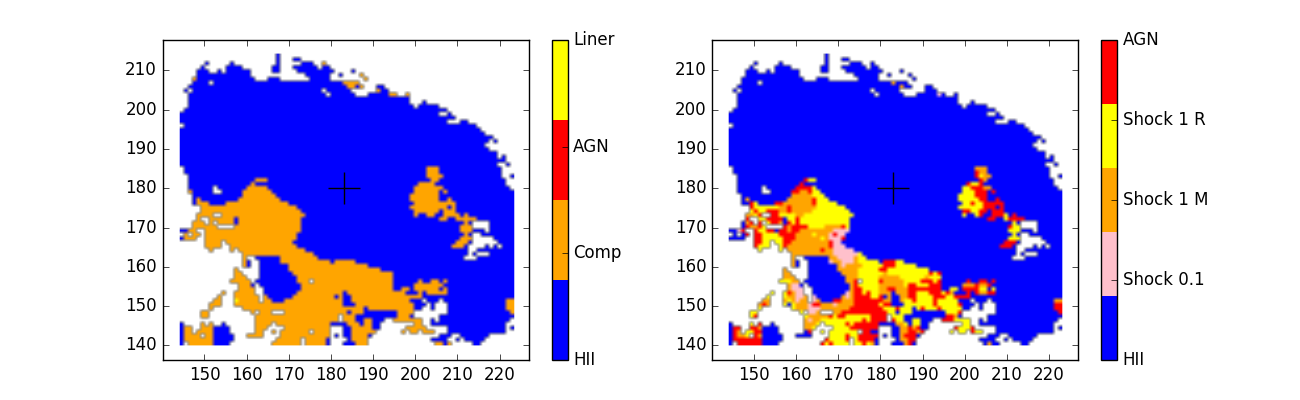
\includegraphics[width=.95\linewidth]{Plots/JO175_NB_xbest_grid.png}\\	
	\end{tabular} 
	\contcaption{}
\end{figure*}


\section{Photoionization and shock model diagrams}
\label{app:VO_diagram}

Fig.\ref{fig:models} displays the observed VO line ratios, color coded with the distance from the center, and overplotted grids of AGN photoionization models (upper row) ans shock models (lower row).

\begin{figure*}
%what to show here: upper row distance color-coded VOs, 
%lower row + shock models [NB maps]
\begin{tabular}{c}
%(a) JO135 \\
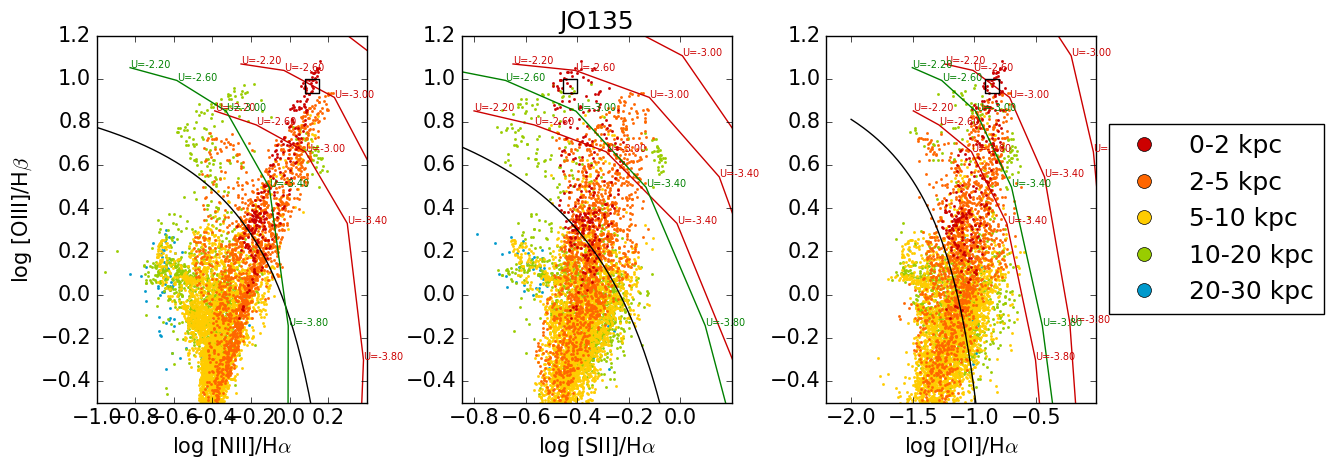
\includegraphics[width=.8\linewidth]{Plots/JO135_vo_dist_NLR.png}\\
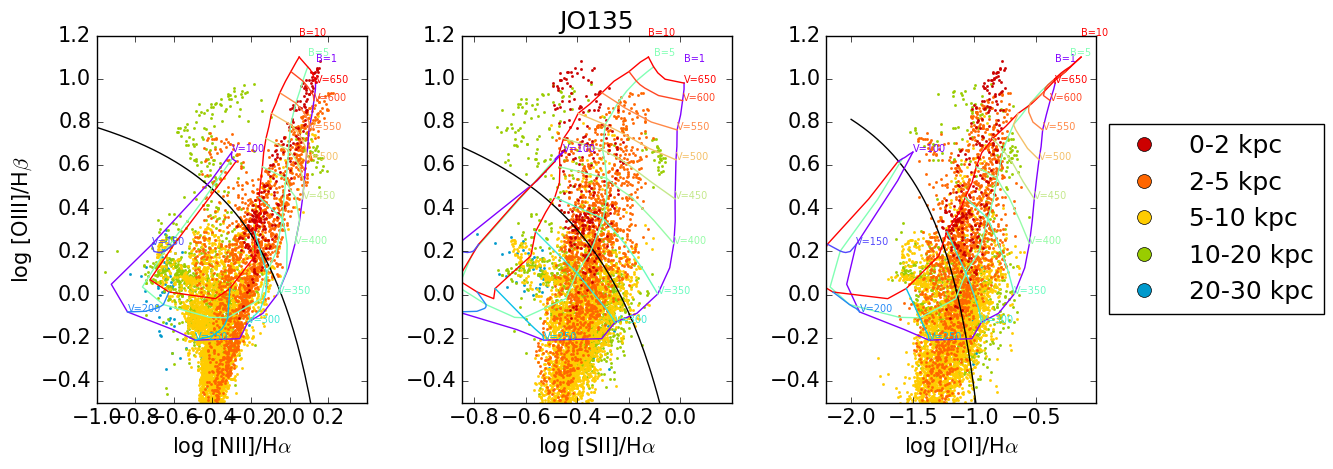
\includegraphics[width=.8\linewidth]{Plots/JO135_vo_dist_SH_n1_R.png}\\
%(b) JO201 \\
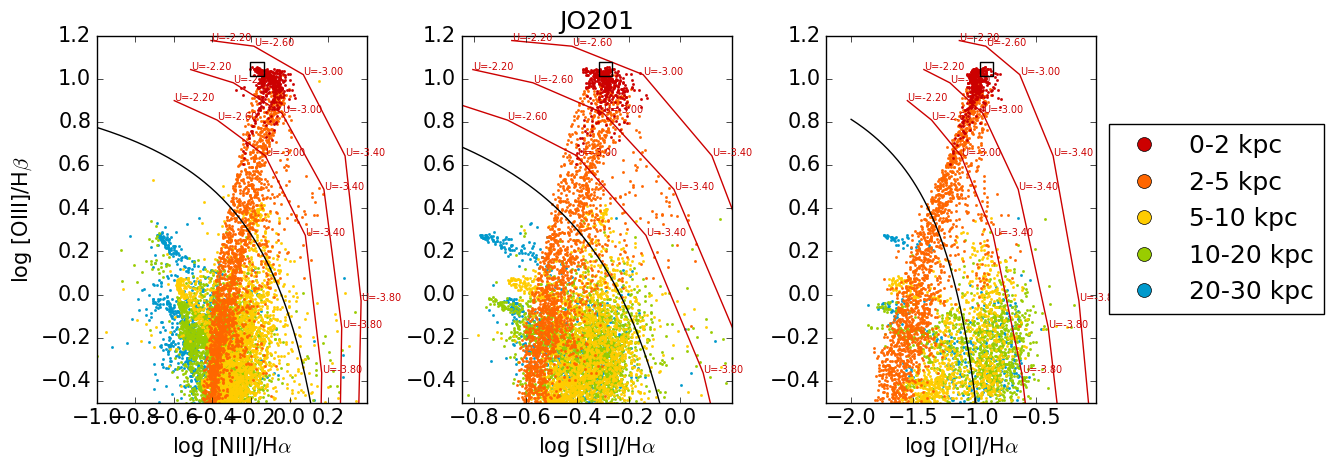
\includegraphics[width=.8\linewidth]{Plots/JO201_vo_dist_NLR.png}\\
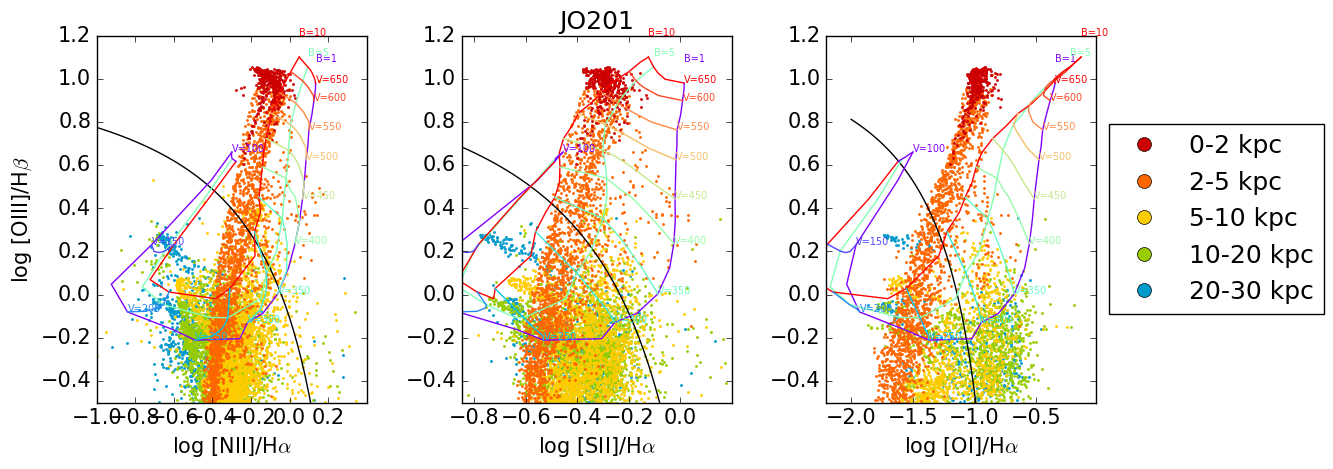
\includegraphics[width=.8\linewidth]{Plots/JO201_vo_dist_SH_n1_R.png}\\

\end{tabular} 
\caption{Observed emission line ratios color coded with the distance from the galaxy center; the empty square displays the value measured in the central spaxel.	
	For each galaxy, overlaid are best-fit AGN (upper row, not for JO175) and shock models (lower row). AGN models are displayed for different values of $U$, best-fit values of $\log P/k$ and $12 + \log O/H$, and  $E_{\rm peak}$ + (-0.25,0,0.25). Shock models are displayed for $n=0.1$ cm$^{-3}$, solar metallicity (JO135, JO201, JO204, JO206);  $n=1$ cm$^{-3}$, 2x solar metallicity (JW100, JO175, JO194). \label{fig:models}}
\end{figure*}

\begin{figure*}
	%what to show here: upper row distance color-coded VOs, 
	%lower row + shock models [NB maps]
	\begin{tabular}{c}
%		(c) JO204 \\
		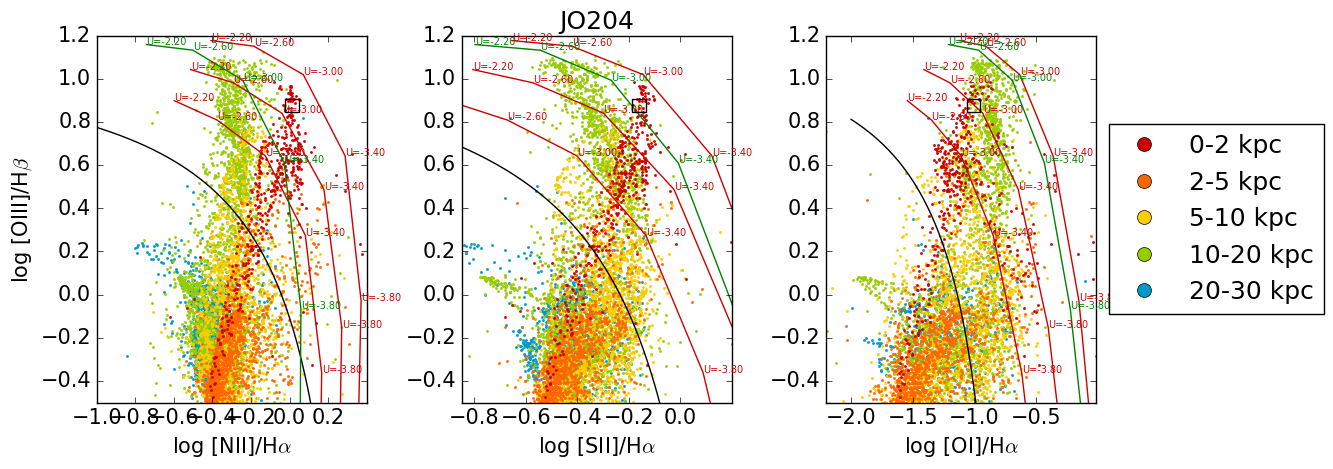
\includegraphics[width=.8\linewidth]{Plots/JO204_vo_dist_NLR.png}\\
		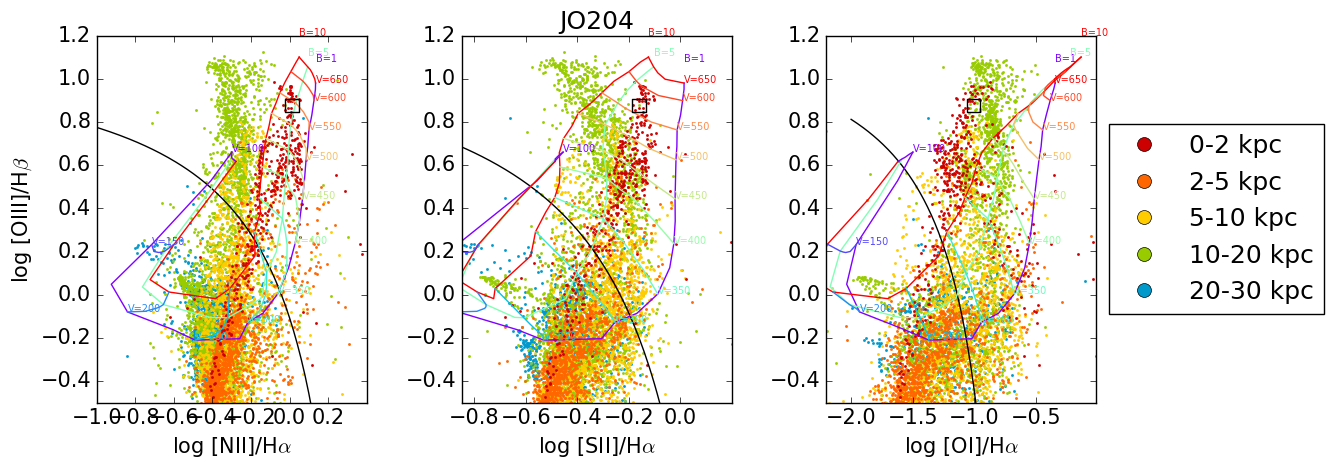
\includegraphics[width=.8\linewidth]{Plots/JO204_vo_dist_SH_n1_R_tot.png}\\
%		(c) JO206 \\		
		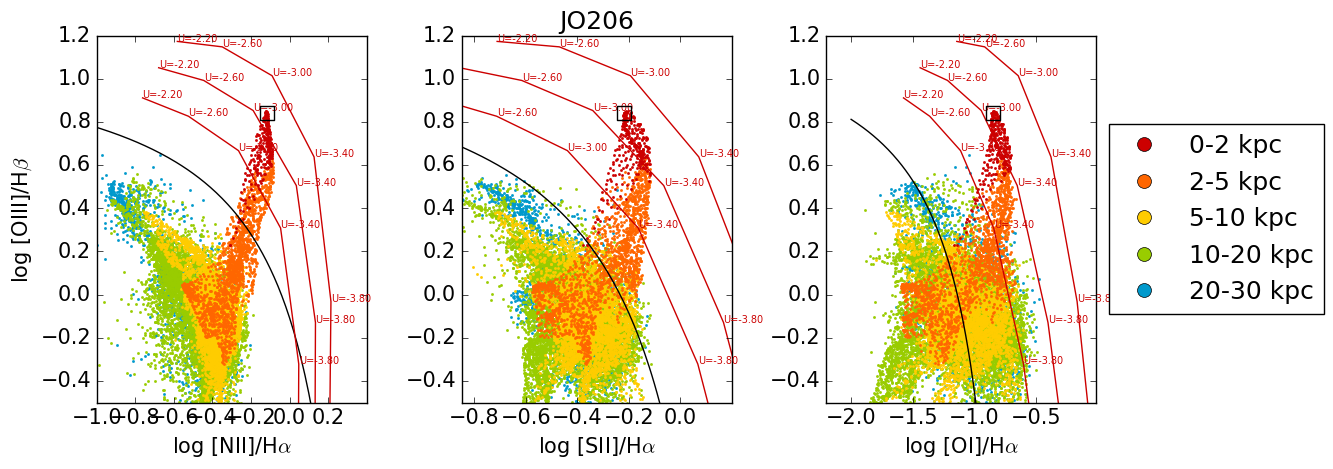
\includegraphics[width=.8\linewidth]{Plots/JO206_vo_dist_NLR.png}\\
		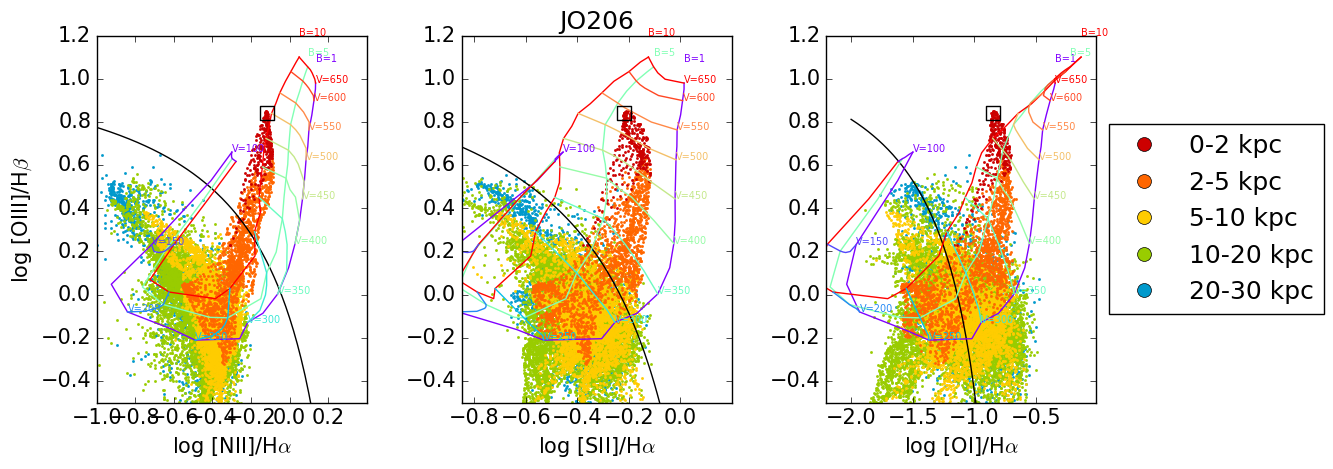
\includegraphics[width=.8\linewidth]{Plots/JO206_vo_dist_SH_n1_R_tot.png}\\
	\end{tabular} 
	\contcaption{}
\end{figure*}

\begin{figure*}
	%what to show here: upper row distance color-coded VOs, 
	%lower row + shock models [NB maps]
	\begin{tabular}{c}
%		(d) JW100 \\
		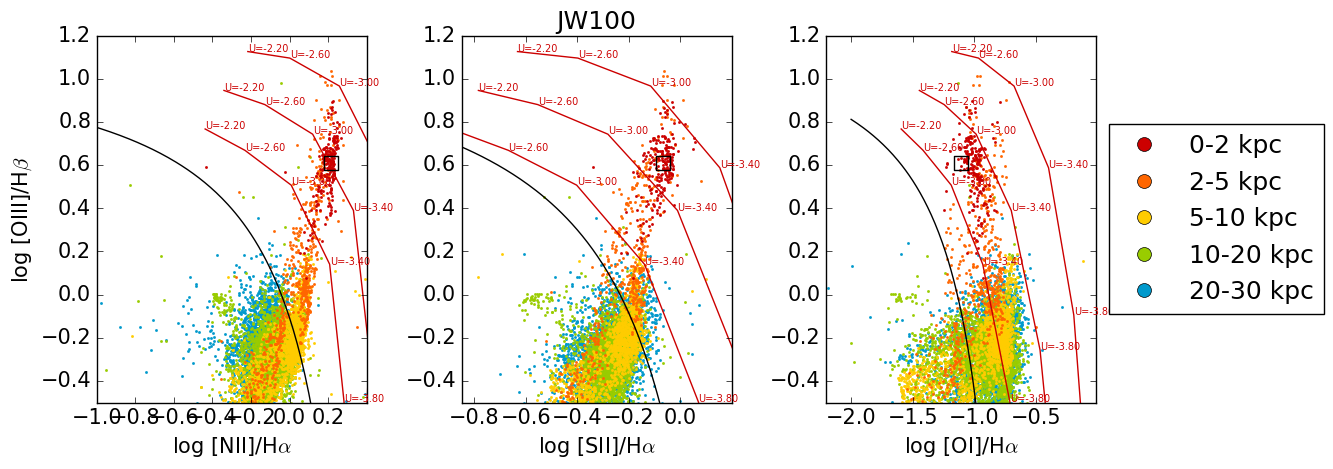
\includegraphics[width=.8\linewidth]{Plots/JW100_vo_dist_NLR.png}\\
		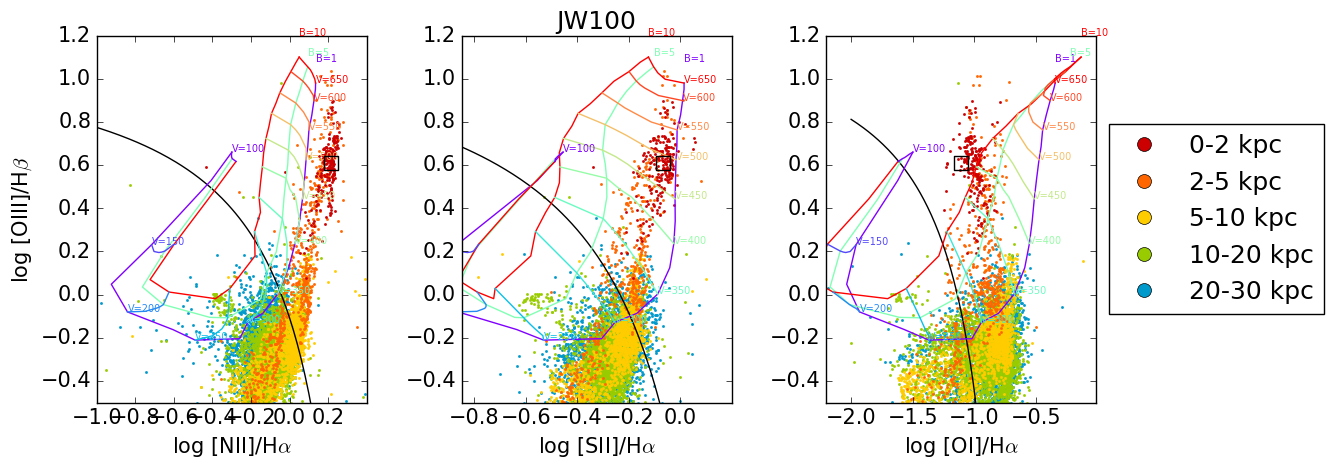
\includegraphics[width=.8\linewidth]{Plots/JW100_vo_dist_SH_n1_R_tot.png}\\
%		(e) JO194 \\		
		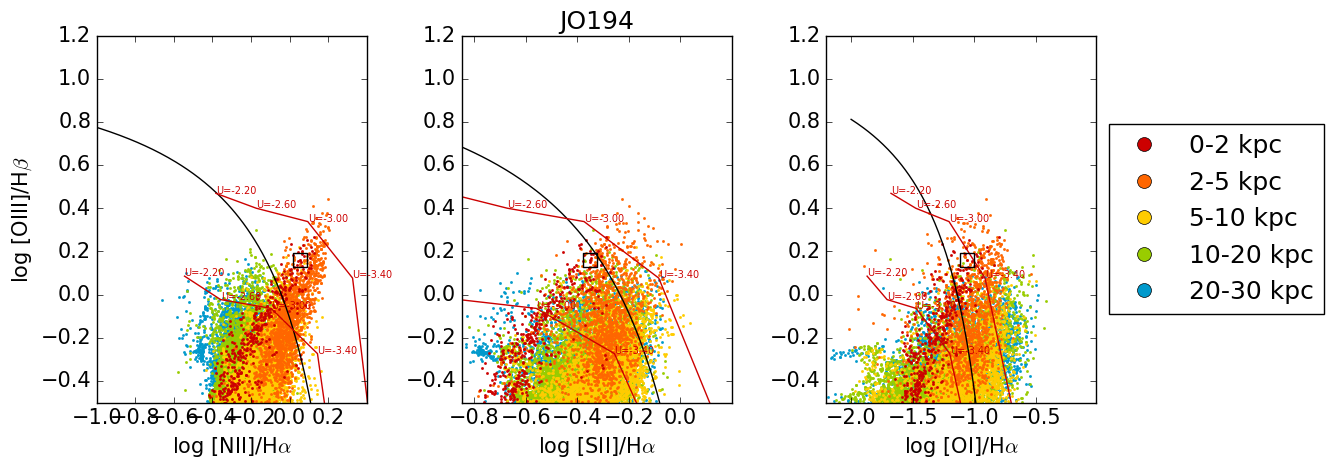
\includegraphics[width=.8\linewidth]{Plots/JO194_vo_dist_NLR.png}\\
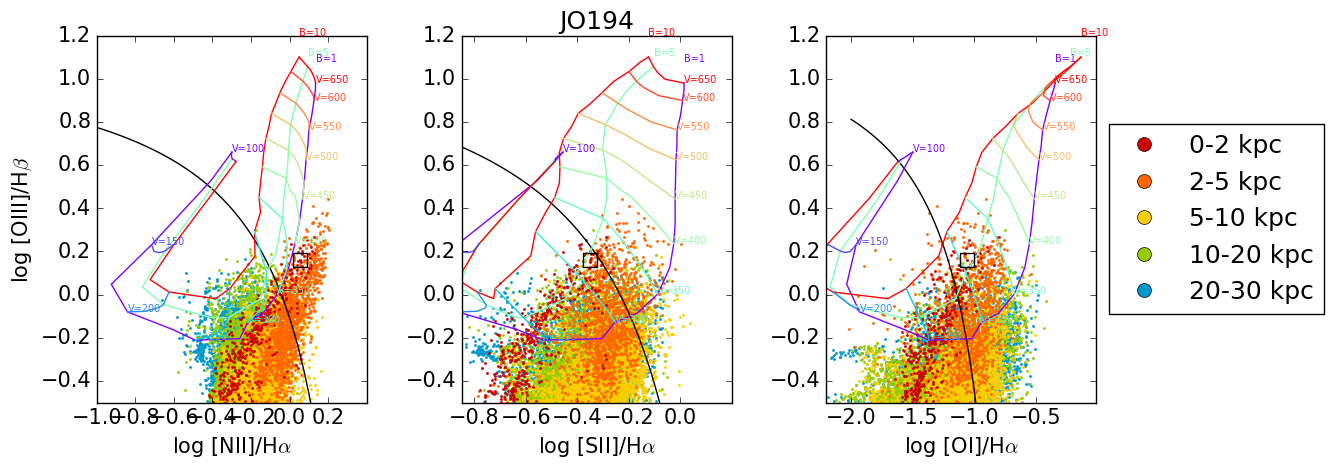
\includegraphics[width=.8\linewidth]{Plots/JO194_vo_dist_SH_n1_R_tot.png}\\
	\end{tabular} 
	\contcaption{}
\end{figure*}

\begin{figure*}
	%what to show here: upper row distance color-coded VOs, 
	%lower row + shock models [NB maps]
	\begin{tabular}{c}%		(f) JO175\\
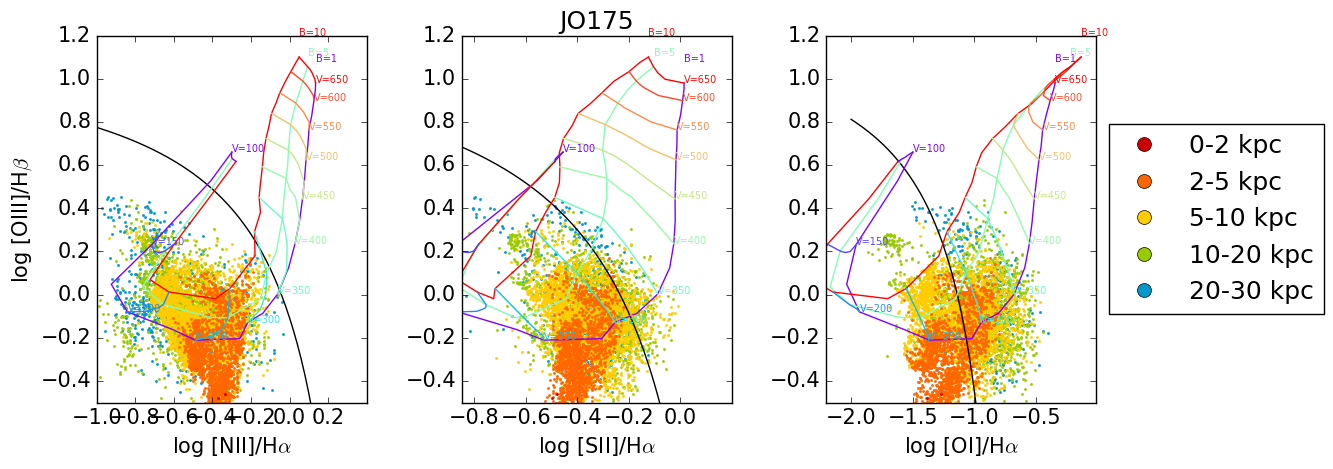
\includegraphics[width=.8\linewidth]{Plots/JO175_vo_dist_SH_n1_R_tot.png}\\
\end{tabular} 
\contcaption{}
\end{figure*}


%\begin{figure*}
%	\begin{tabular}{cc}
%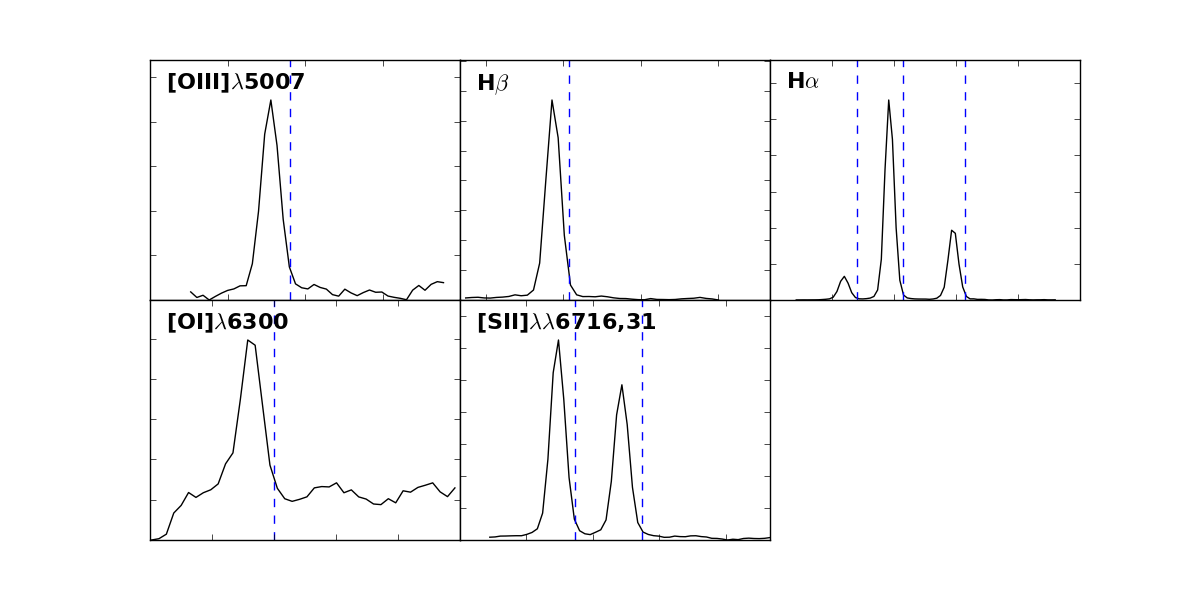
\includegraphics[width=1\linewidth]{Plots/alines_peak_JO175} & 
%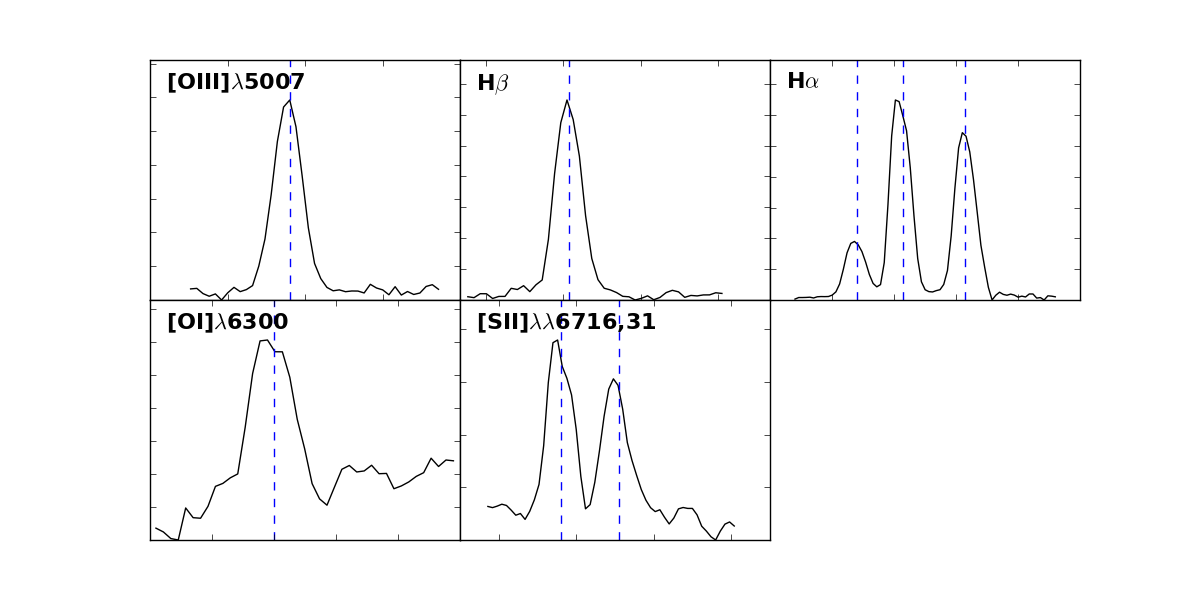
\includegraphics[width=1\linewidth]{Plots/alines_peak_JO194} &\\
%	\end{tabular} 
%	\caption{One-component emission line fits in the central spaxel (JO175, JO194)}
%\end{figure*}




\section{Spatial distribution of non-parametric measurements.}
\label{app:map_nonparam}

For the galaxies showing outflow signatures, 
Fig.\ref{fig:npars} displays the spatial distribution of the non-parametric measurements $v_{\rm peak}$, $W_{80}$,  $A_{\rm sym}$ defined in Sect.\ref{sect:Outflows}. In each row, the first panel shows for comparisons the spatial distribution of the stellar velocity.

\begin{figure*}
	\begin{tabular}{c}
		JO135 \\
		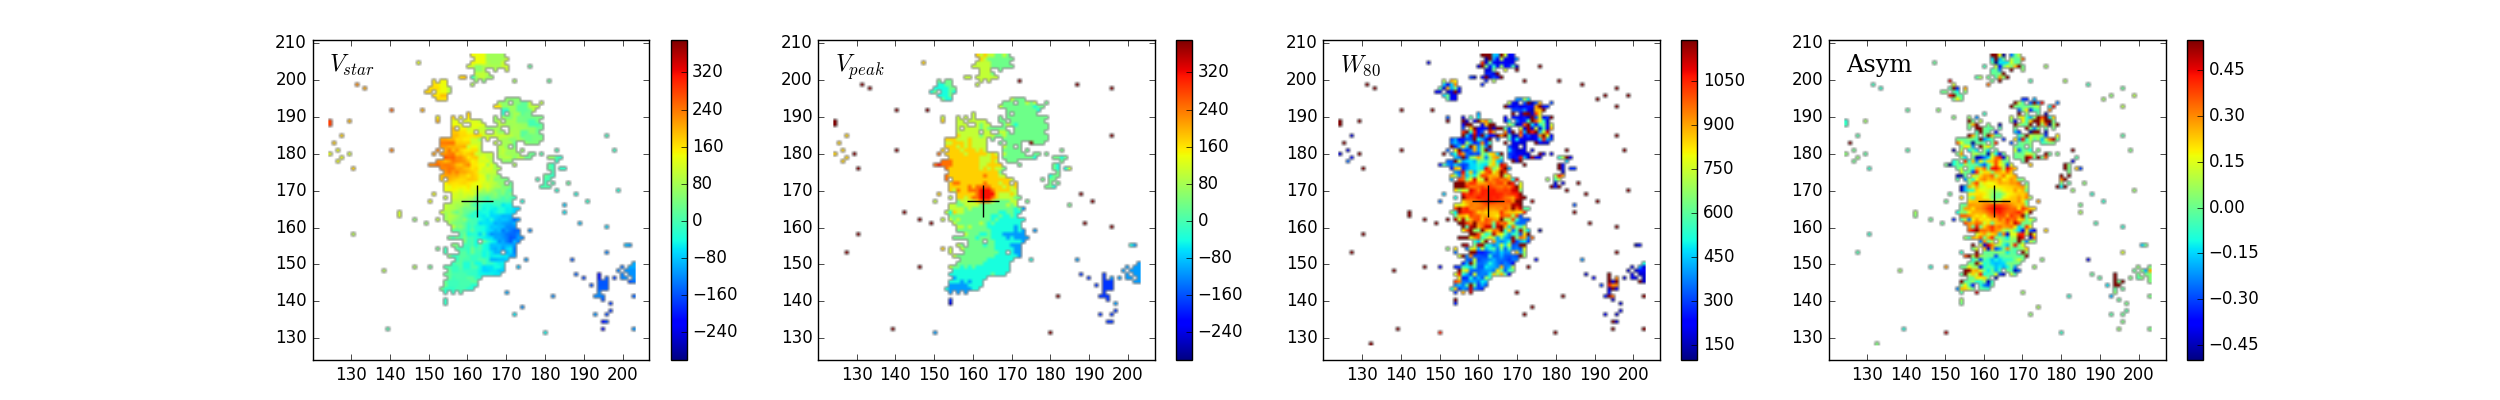
\includegraphics[width=.9\linewidth]{Plots/JO135_npars_grid.png}\\
		JO201 \\
		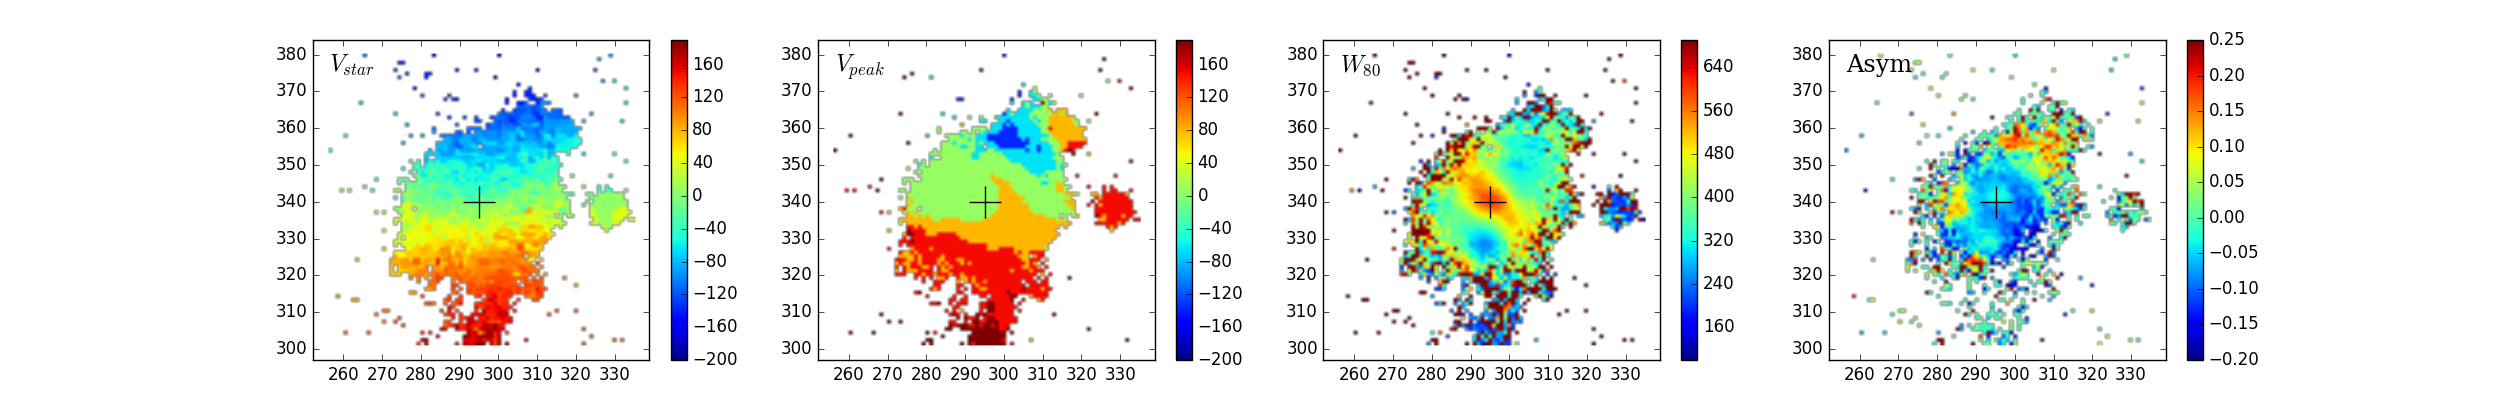
\includegraphics[width=.9\linewidth]{Plots/JO201_npars_grid.png} \\
		JO204\\
		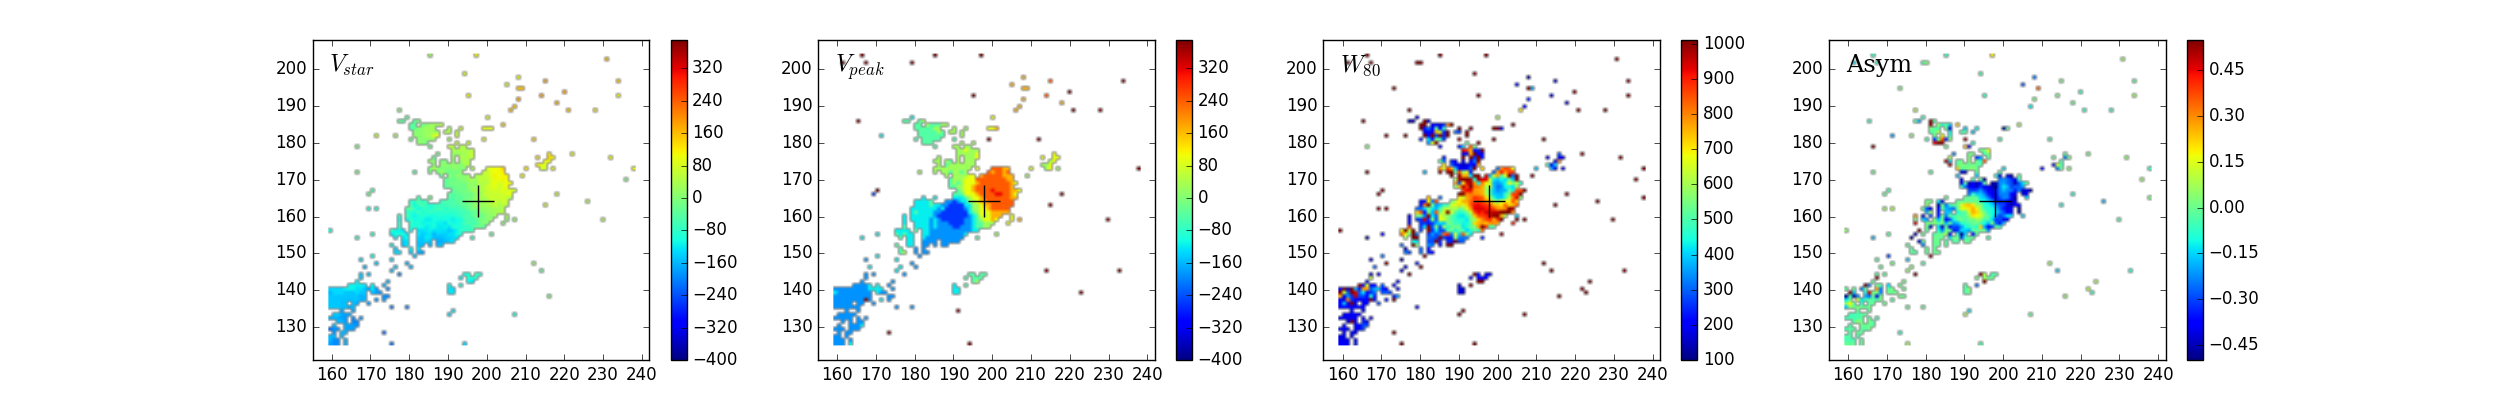
\includegraphics[width=.9\linewidth]{Plots/JO204_npars_grid.png}\\
		JO206\\
		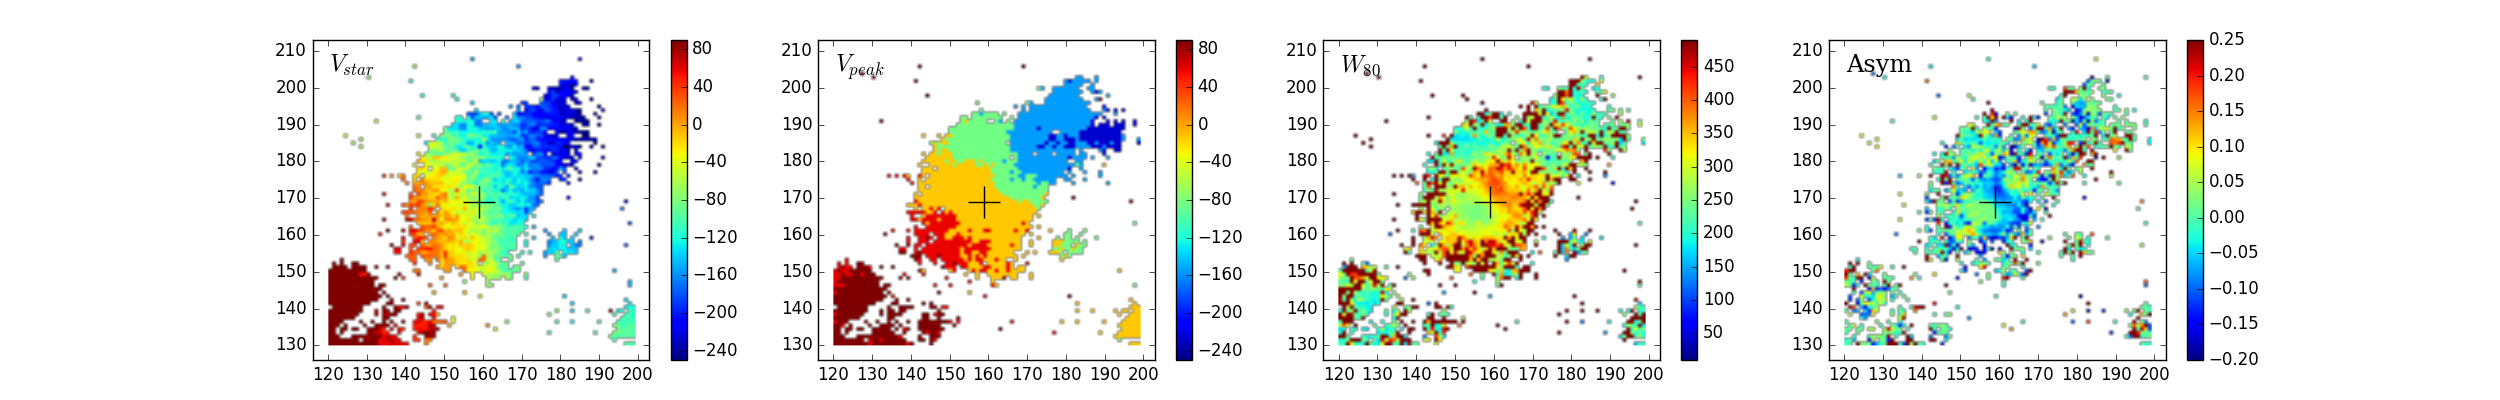
\includegraphics[width=.9\linewidth]{Plots/JO206_npars_grid.png}\\
		JW100\\
		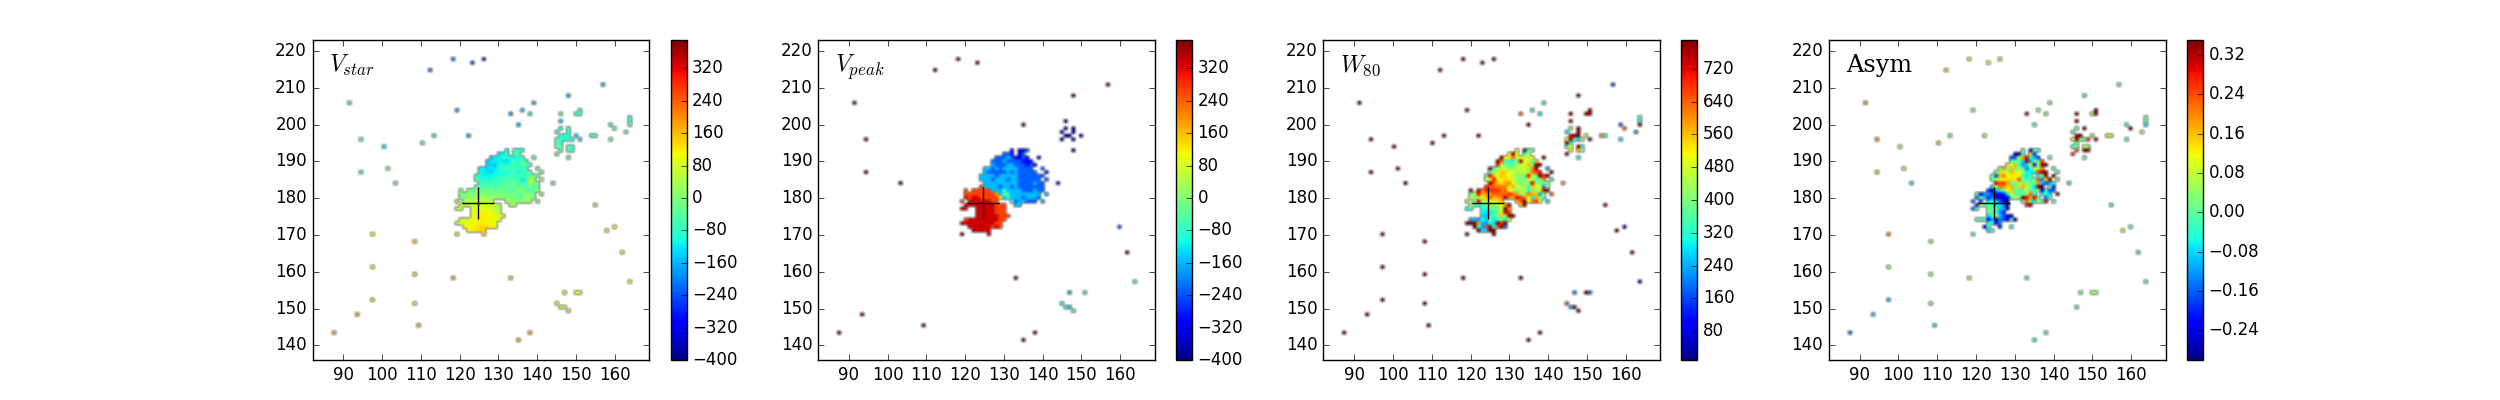
\includegraphics[width=.9\linewidth]{Plots/JW100_npars_grid.png}\\
	\end{tabular} 
	\caption{For each galaxy hosting an AGN, the plots display the spatial distribution  of the stellar velocity [km/s] (first panel) and of the following parameters (see text for details) derived from the [OIII] line: peak velocity [km/s] ({\em left panel});
	$W_{\rm 80}$ [km/s] ({\em middle panel}); asymmetry ({\em right panel}). In each plot, North is up and East is at left.\label{fig:npars}}
\end{figure*}


\section{Spatial distribution of parametric measurements.}
\label{app:map_param}

For the galaxies showing outflow signatures, 
Fig.\ref{fig:fpars} show for the narrow and broad component the  spatial distribution of the velocity dispersion ($\sigma_v$) and the VO ratios ([NII]$\lambda$6583/H$\alpha$, [SII]$\lambda\lambda$6716,6731/H$\alpha$, [OI]$\lambda$6300/H$\alpha$ vs. [OIII]$\lambda$5007/H$\beta$).

\begin{figure*}
	\begin{tabular}{c}
		JO135 \\
		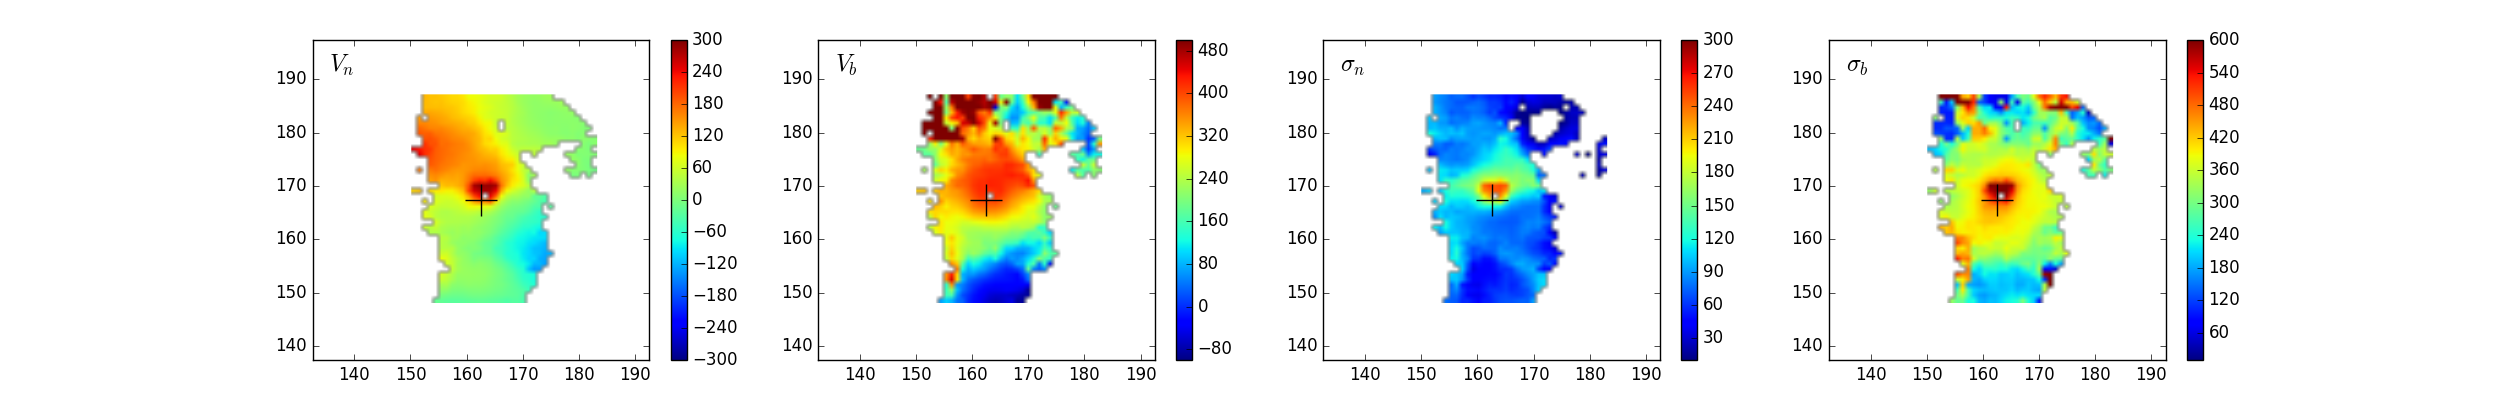
\includegraphics[width=1\linewidth]{Plots/JO135_fpars_kin.png}\\		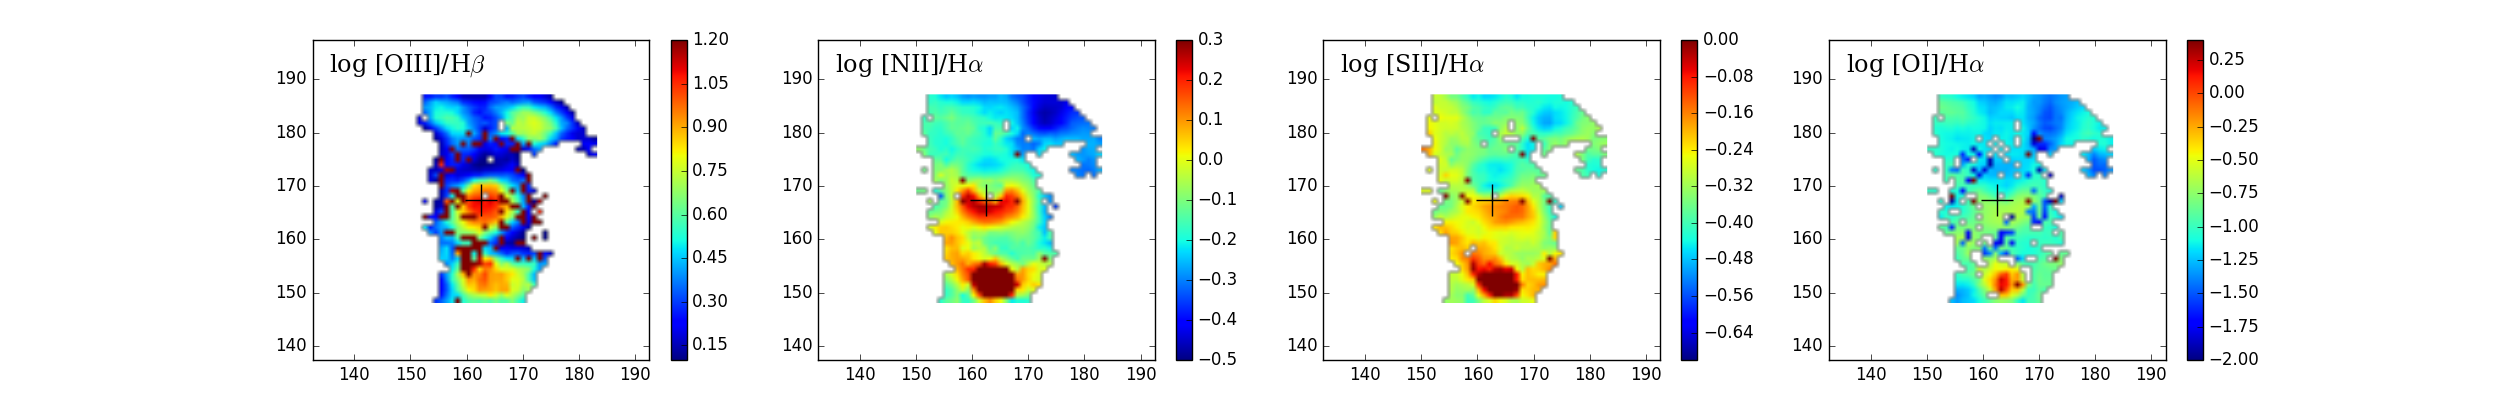
\includegraphics[width=1\linewidth]{Plots/JO135_fpars_n.png}\\
		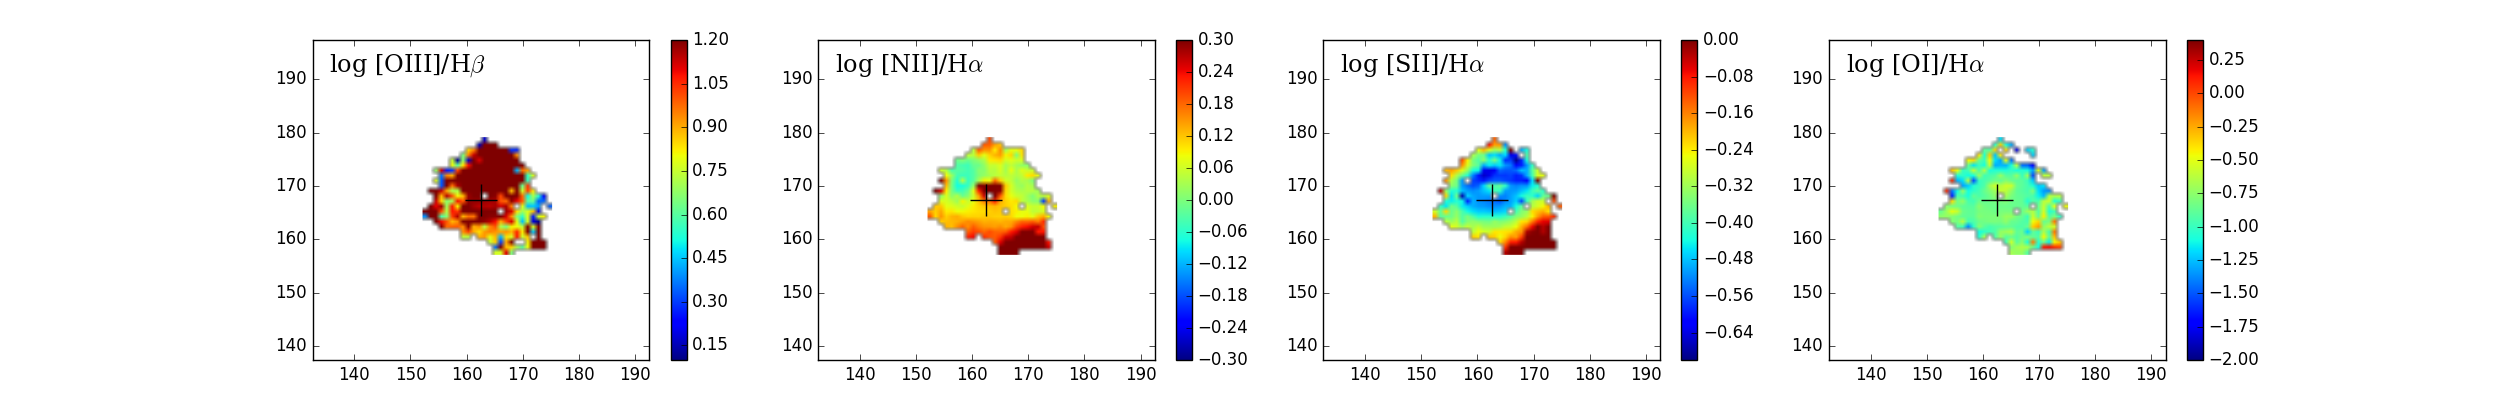
\includegraphics[width=1\linewidth]{Plots/JO135_fpars_b.png}\\
		JO201 \\
		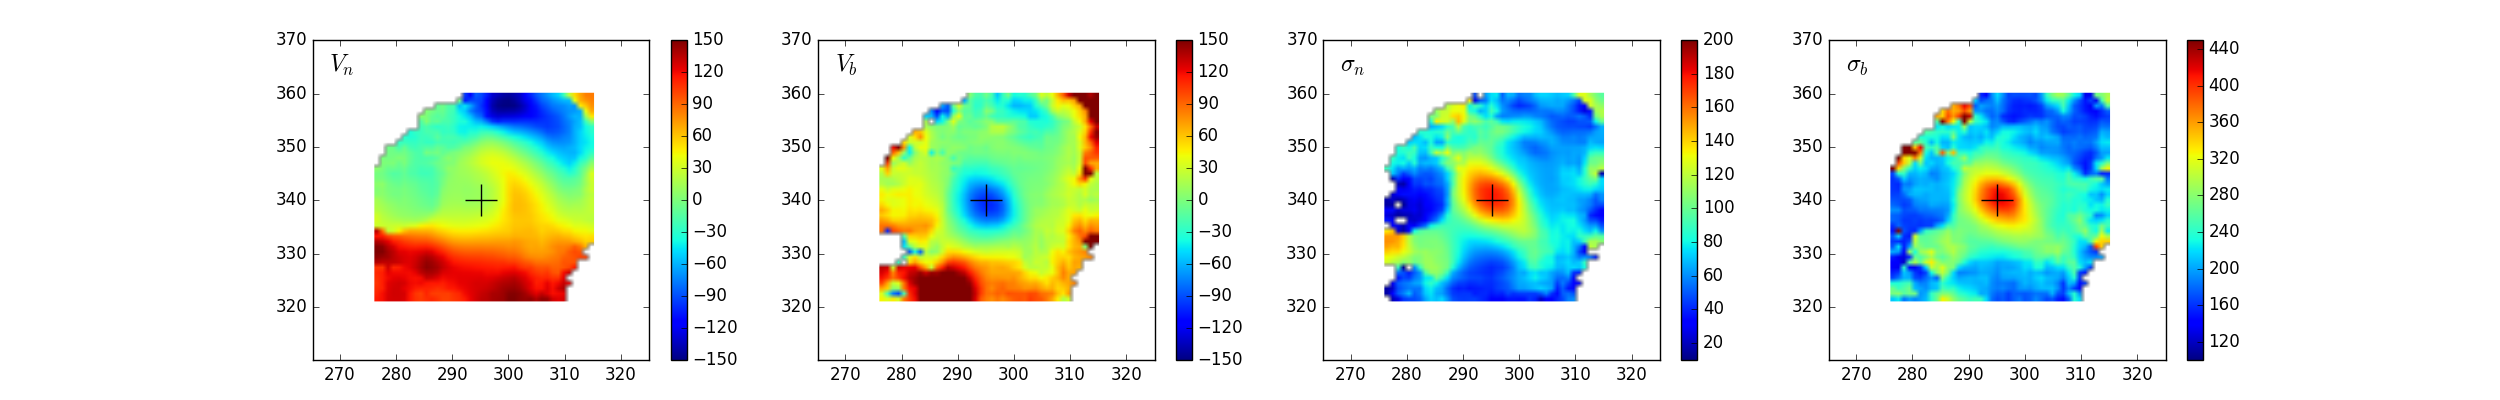
\includegraphics[width=1\linewidth]{Plots/JO201_fpars_kin.png} \\		\includegraphics[width=1\linewidth]{Plots/JO201_fpars_n.png} \\
		\includegraphics[width=1\linewidth]{Plots/JO201_fpars_b.png} \\
		%
%		JO206\\
%		\includegraphics[width=1\linewidth]{Plots/JO206_fpars_b.png}\\		
	\end{tabular} 
	\caption{Results obtained from the line fitting based on [OIII]$\lambda$5007.\label{fig:fpars}}
\end{figure*}

\begin{figure*}
	\begin{tabular}{c}
		JO204\\
		\includegraphics[width=1\linewidth]{Plots/JO204_fpars_kin.png}\\
		\includegraphics[width=1\linewidth]{Plots/JO204_fpars_n.png}\\
		\includegraphics[width=1\linewidth]{Plots/JO204_fpars_b.png}\\		
		JW100\\
		\includegraphics[width=1\linewidth]{Plots/JW100_fpars_kin.png}\\
		\includegraphics[width=1\linewidth]{Plots/JW100_fpars_n.png}\\
%		\includegraphics[width=1\linewidth]{Plots/JW100_fpars_b.png}\\		
		%
		%		JO206\\
		%		\includegraphics[width=1\linewidth]{Plots/JO206_fpars_b.png}\\		
	\end{tabular} 
	\contcaption{}
\end{figure*}

%\begin{figure*}
%	\begin{tabular}{cc}
%		JO135 & JW100\\
%		\includegraphics[width=.5\linewidth]{Plots/JO135_nb_vo.png}& 
%		\includegraphics[width=.5\linewidth]{Plots/JW100_nb_vo.png}\\
%		JO201 & JO204\\
%		\includegraphics[width=.5\linewidth]{Plots/JO201_nb_vo.png} &
%		\includegraphics[width=.5\linewidth]{Plots/JO204_nb_vo.png}\\
%		JO206\\		
%		\includegraphics[width=.5\linewidth]{Plots/JO206_nb_vo.png}\\
%	\end{tabular} 
%	\caption{Line ratios obtained from the broad and narrow line decomposition. In the case of JW100, the decomposition refers to the blue and redshifted components, of similar width. \label{fig:vo_nb}}
%\end{figure*}


% Don't change these lines
\bsp	% typesetting comment
\label{lastpage}
\end{document}

% End of mnras_template.tex